\documentclass[11pt]{article}
\usepackage[margin=1in]{geometry}
\usepackage[T1]{fontenc}
\usepackage{lmodern}
\usepackage{amsmath,amssymb,amsthm,mathtools}
\usepackage{bm}
\usepackage{booktabs,multirow,array}
\usepackage{graphicx}
\usepackage{xcolor}
\usepackage{tikz}
\usetikzlibrary{arrows.meta,positioning,fit,calc,shapes.geometric}
\usepackage{siunitx}
\usepackage{algorithm}
\usepackage{algpseudocode}
\usepackage[numbers,sort&compress]{natbib}
\usepackage[colorlinks=true,linkcolor=blue!50!black,citecolor=blue!50!black,urlcolor=blue!50!black]{hyperref}
\usepackage[capitalise,noabbrev]{cleveref}

\newtheorem{proposition}{Proposition}
\newtheorem{lemma}{Lemma}
\newtheorem{remark}{Remark}
\theoremstyle{definition}
\newtheorem{definition}{Definition}

% Shared notation (paper/BRIEF.md §3). Use these macros; do not redefine them in a section.
\makeatletter
% \X_{..} after a macro that already carries a subscript joins the two: \Mdiv_{ij} -> M_{div,ij}.
\newcommand{\@joinsub}[2]{\@ifnextchar_{\@joinsub@{#1}{#2}}{#1_{#2}}}
\def\@joinsub@#1#2_#3{#1_{#2,#3}}
\makeatother
\newcommand{\R}{\mathbb{R}}
\newcommand{\Omegac}{\Omega}                       % cavity volume
\newcommand{\bdry}{\partial\Omega}                 % PEC wall
\newcommand{\E}{\mathbf{E}}
\newcommand{\Hf}{\mathbf{H}}
\newcommand{\curl}{\nabla\times}
\newcommand{\Hcurl}{H_0(\mathrm{curl};\Omega)}
\newcommand{\Vh}{V_h}                              % discrete H(curl) space (Nedelec, order p, curved mesh)
\newcommand{\Sh}{S_h}                              % discrete H^1_0 potential space, order p+1
\newcommand{\Kmat}{\mathsf{K}}                     % curl-curl stiffness
\newcommand{\Mmat}{\mathsf{M}}                     % mass
\newcommand{\Gmat}{\mathsf{G}}                     % discrete gradient (potentials -> H(curl) DOFs)
\makeatletter\DeclareRobustCommand{\Kp}{\@joinsub{\mathsf{K}}{p}}\makeatother                     % G^T M G
\newcommand{\Pmat}{\mathsf{P}}                     % kernel projection
\newcommand{\Vmat}{\mathsf{V}}                     % learned basis in DOFs, n x m
\newcommand{\Cmat}{\mathsf{C}}                     % fixed point-values -> DOF map
\makeatletter\DeclareRobustCommand{\Mdiv}{\@joinsub{\mathsf{M}}{\mathrm{div}}}\makeatother
\makeatletter\DeclareRobustCommand{\Av}{\@joinsub{\mathsf{A}}{V}}\makeatother
\newcommand{\ndof}{n}
\newcommand{\nbasis}{m}                            % width of the learned basis
\newcommand{\nmodes}{K}                            % number of predicted modes
\makeatletter\DeclareRobustCommand{\lamh}{\@joinsub{\lambda}{h}}\makeatother  % discrete eigenvalue; \lamh_k -> lambda_{h,k}
\makeatletter\DeclareRobustCommand{\Qz}{\@joinsub{Q}{0}}\makeatother
\newcommand{\RoQ}{R/Q}
\makeatletter\DeclareRobustCommand{\Epk}{\@joinsub{E}{\mathrm{pk}}}\makeatother
\makeatletter\DeclareRobustCommand{\Bpk}{\@joinsub{B}{\mathrm{pk}}}\makeatother
\makeatletter\DeclareRobustCommand{\Eacc}{\@joinsub{E}{\mathrm{acc}}}\makeatother
\makeatletter\DeclareRobustCommand{\Lacc}{\@joinsub{L}{\mathrm{acc}}}\makeatother
\newcommand{\LF}{\mathrm{LF}}
\newcommand{\HF}{\mathrm{HF}}
\newcommand{\relLtwo}{\mathrm{rel\text{-}L^2}}
\DeclareMathOperator{\spn}{span}
\DeclareMathOperator{\diag}{diag}


\title{Rayleigh--Ritz Neural Operators for the Resonant Modes of 3D RF Cavities:\\
Discrete Upper-Bound Eigenvalues on Curved High-Order Elements and Training with Low-Fidelity Labels}
\author{Author names to be added}
\date{}

\begin{document}
\maketitle

\begin{abstract}
Predicting the resonant modes of three-dimensional radio-frequency (RF) cavities---their frequencies, electric
fields and figures of merit such as $\Qz$, $\RoQ$ and the peak surface fields---normally requires one
finite-element eigensolve per geometry. We present a neural operator that does not regress these quantities
directly. It maps the geometry, represented by the quadrature points of a curved tetrahedral mesh, to a learned
basis of vector fields; a fixed linear map turns the basis into degrees of freedom of a second-order N\'ed\'elec
space, a kernel projection removes the discrete gradients, and a Rayleigh--Ritz step returns the modes. The
predicted eigenvalues are therefore upper bounds of the discrete eigenvalues of whichever conforming space the
model runs in, and no spurious zero modes arise. Single-sample fits reach relative eigenvalue errors of
$10^{-6}$--$9\times10^{-6}$. % src: docs/28 §3
We build an adaptive third-order label generator on curved meshes, validated against analytic pillbox modes
(relative frequency error $6\times10^{-7}$ at 157k degrees of freedom), % src: docs/31 §1
and show that low-fidelity labels---one second-order solve on the same model mesh---cost $4.3\times$ less
while differing from the adaptive labels by at most $0.047\,\%$ in frequency and $0.32\,\%$ in field. % src: docs/34 §8.1
In a controlled small-scale study on one cavity family, models trained on low-fidelity labels were at least as
accurate on held-out high-fidelity geometries as models trained on high-fidelity labels of equal or higher
cost, and their errors against low- and high-fidelity labels differ by $0.02$ percentage points. % src: docs/34 §8.2

\end{abstract}

\section{Introduction}\label{sec:introduction}

For a superconducting accelerator cavity such as the nine-cell \SI{1.3}{GHz} niobium structure of the TESLA design \citep{aune2000superconducting,padamsee2009rf},
the designer needs the mode frequencies, the fields and the derived figures of merit:
the unloaded quality factor $\Qz$, the shunt impedance $\RoQ$, and the
peak-field ratios $\Epk/\Eacc$ and $\Bpk/\Eacc$ that limit the achievable gradient.
Each design iteration changes the shape and needs a new three-dimensional eigenvalue solve on a curved geometry.
Axisymmetric codes \citep{halbach1976superfish} are cheap but cover only part of the design space;
general three-dimensional design relies on finite-element eigensolvers such as the ACE3P suite \citep{ko2010advances} or commercial tools such as CST Studio Suite,
whose cost per geometry grows with the mesh resolution needed for accurate figures of merit.
A surrogate that returns frequencies, fields and figures of merit directly from the geometry would shorten the loop,
provided it can be trusted at the accuracy of the solver it replaces.

Neural operators \citep{lu2021learning,li2021fourier,kovachki2023neural}, which learn the map from a PDE's input to its solution, are natural candidates.
Applying them directly to the Maxwell eigenproblem $\curl\curl\,\E=k^2\E$ in $\Omega$ with $\mathbf{n}\times\E=0$ on $\partial\Omega$ is problematic for three reasons.
First, the network must return an ordered set of modes with mutually consistent eigenvalues and fields, and a plain regression loss guarantees none of this.
Second, the curl operator has an infinite-dimensional kernel formed by gradient fields;
any discretisation that does not respect the $H(\mathrm{curl})$ structure, and any predicted field that is not projected away from this kernel,
produces spurious modes at or near zero frequency \citep{hiptmair2002finite,boffi2010finite}.
Third, a network that outputs values on a fixed grid or degrees of freedom is tied to one discretisation, whereas eigenvalue accuracy depends on the mesh and the polynomial order.

\paragraph{Approach.}
We therefore do not ask the network for the modes themselves.
The network maps the geometry to a \emph{learned basis} of $m$ vector fields ($m$ is the basis width; $K\le m$ denotes the number of predicted modes).
A fixed linear map takes the basis to the degrees of freedom of a conforming high-order N\'ed\'elec space \citep{nedelec1980mixed} of order $p$ on a curved (isoparametric) mesh,
the basis is projected onto the discretely divergence-free subspace (the kernel projection, a float64 conjugate-gradient solve),
and a Rayleigh--Ritz step in the projected span returns the $K$ lowest frequencies and the fields.
The network is trained mainly to place the true modes inside the span of the basis; the Ritz step, not a regression head, computes frequencies and fields, and as a Galerkin projection it obeys min--max.
We implement it with NGSolve and Netgen \citep{schoberl1997netgen,schoberl2014cpp11}.

\paragraph{Contributions.}
\begin{enumerate}
  \item \textbf{A neural operator with a built-in discrete eigenvalue bound.}
  Every predicted eigenvalue bounds from above the corresponding nonzero discrete eigenvalue of the space in which the model runs,
  and the kernel projection excludes spurious zero modes (\cref{sec:method}, \cref{prop:upper-bound}).
  In the main held-out study every prediction stayed above the discrete eigenvalue of its space (smallest margin $f_{\mathrm{model}}/f_{\mathrm{FE}}-1=\SI{0.47}{\percent}$ over arms, geometries and modes); % src: docs/34 §8.2
  the bound is relative to the discrete, not the exact, eigenvalue and does not certify mode identity.
  % TODO pass 3: rank check of assumption (A) and Ritz-bound stress test with the a posteriori inexact-CG bound
  \item \textbf{Independence of the discretisation space.}
  The same weights run unchanged on a $p=3$ space and on a mesh refined once ($8\times$ tetrahedra); all predicted eigenvalues lay above the FE eigenvalue of the evaluated space. % src: docs/34 §4.2
  Accuracy does not improve there (frequency error up by \numrange{0.2}{0.7} percentage points), which we attribute, untested, to the learned basis. % src: docs/34 §4.2, referee E6
  \item \textbf{Single-sample representation capacity.}
  With quadrature-point tokens on a curved $p=2$ space, fitting one 179-tetrahedron sample to its own $p=2$ label reaches a relative eigenvalue error of \numrange{1e-6}{9e-6}. % src: docs/28 §3
  This shows the representation can express the modes, not that it generalises.
  \item \textbf{A data pipeline with analytic validation.}
  An adaptive $p=3$ label generator on curved meshes (\cref{sec:data}); on an analytic smooth pillbox (no pipes or fillets) it reproduces the exact values to \num{6e-7} in frequency, \num{3e-5} in $\Qz$, \num{1e-5} in $\RoQ$, \num{2e-4} in $\Epk$ and \num{4e-4} in $\Bpk$ at \num{157000} degrees of freedom. % src: docs/31 §1
  Removing repeated work cut an adaptive label at \num{450000} DOF from \SI{664}{s} to \SI{433}{s}. % src: docs/31 §3.8
  \item \textbf{Training on low-fidelity labels.}
  A low-fidelity (LF) label is one $p=2$ solve on the model mesh. The high-fidelity (HF) label used in all training experiments is one $p=3$ solve on the same start mesh, projected to $p=2$; the adaptive generator path is not exercised by these experiments (\cref{sec:multifidelity}). % src: referee E2, EDITOR_NOTES_2 decision 3
  On this mesh an LF label is $2.8$--$4.3\times$ cheaper (the range reflects machine load), % src: docs/34 §8.1, EDITOR_NOTES_2 decision 4
  differs from the HF label by \SIrange{0.004}{0.047}{\percent} in frequency and \SIrange{0.08}{0.32}{\percent} (mass norm) in the field subspace, % src: docs/34 §8.1
  and the model's errors measured against LF and against HF labels differ by only $0.02$ percentage points. % src: docs/34 §8.2
  In an equal-cost comparison on six held-out HF geometries, LF-trained and HF-trained models reached comparable accuracy (\cref{tab:equal-cost}).
  Limits: single runs; fidelity and the number of training geometries change together (no LF run on the HF geometries); and the label difference is one to two orders of magnitude smaller than the model error, so the study does not yet probe the regime where label type matters. % src: referee E1, EDITOR_NOTES_2 decision 2
  % TODO pass 3: repeated seeds / LF-8 control if produced; parametric-regression and coarse-FE baselines
\end{enumerate}

\paragraph{Scope.}
This is a method-and-pipeline paper with small-scale evidence: CPU training, at most 40 training geometries from one family (a pillbox with beam pipes), a 64-dimensional two-block trunk. % src: BRIEF §1; docs/34 §4, §8.2
The absolute frequency errors of \SIrange{1}{2}{\percent} reflect this under-trained model, not a limit of the method;
the figure-of-merit loss is off; fine-tuning on HF labels and mixed LF+HF training were inconclusive (\cref{sec:experiments}).
Single-threaded, the model path takes \SI{8.3}{s} (operators \SI{5.0}{s}, forward pass \SI{3.3}{s}) against \SI{18}{s} to assemble and solve the FE problem in the same space; % src: docs/34 §8.2, EDITOR_NOTES_2 decision 7
at these sizes this is about a factor of two, not a speed advantage.
The model cannot beat the FE solution of its own space, and no external baseline (parametric regression, coarse FE) is included yet (\cref{sec:discussion}). % TODO pass 3: baselines

\paragraph{Outline.}
\Cref{sec:related} reviews related work; \cref{sec:formulation} states the eigenproblem; \cref{sec:method} gives the model and the bound;
\cref{sec:data} and \cref{sec:multifidelity} cover the label generator and the two fidelities; \cref{sec:experiments} reports the experiments; \cref{sec:discussion} discusses limitations and future work.

\section{Related work}\label{sec:related}

\paragraph{Neural operators.}
Neural operators learn maps between function spaces: DeepONet splits the approximation into a branch and a trunk network~\citep{lu2021learning}, the Fourier neural operator (FNO) parametrises an integral kernel in Fourier space on regular grids~\citep{li2021fourier}, and \citet{kovachki2023neural} give a general framework with approximation results.
Complex domains are handled either by learning a deformation onto a uniform latent grid (Geo-FNO)~\citep{li2023fourier}, by coupling graph and Fourier operators through a signed-distance representation of the shape (GINO)~\citep{li2023geometry}, or by message passing on the simulation mesh itself~\citep{pfaff2021learning}.
Transformer operators replace the softmax by a linear-complexity attention~\citep{katharopoulos2020transformers}: the Galerkin transformer reads it as a Petrov--Galerkin projection~\citep{cao2021choose}, GNOT adds heterogeneous normalised attention and geometric gating for irregular meshes~\citep{hao2023gnot}, and Transolver attends over learned slices of mesh points~\citep{wu2024transolver}.
Evaluating a trained operator on a discretisation other than the training one is a stated feature of FNO-type models~\citep{li2021fourier}, and aliasing between discretisations has been analysed~\citep{bartolucci2023representation}; our setting differs in that the discretisation is a conforming finite-element space, so transfer across spaces keeps the Ritz structure (\cref{sec:method}).
Our trunk belongs to this last family, with quadrature weights playing the role of the mass.
These models regress the solution field, or a scalar functional of it, at the mesh points.
Ours does not: the network emits a \emph{basis} of $m$ vector fields, and the fields and frequencies are produced by a finite-element Rayleigh--Ritz step, so the output inherits the structure of the discrete problem (\cref{sec:method}).

\paragraph{Learning eigenvalue problems and subspaces.}
Neural eigensolvers parametrise eigenfunctions and minimise a variational or fixed-point objective for \emph{one} operator.
Spectral inference networks learn the leading eigenfunctions of a linear operator by stochastic bilevel optimisation~\citep{pfau2019spectral}, and NeuralEF does so for kernels without an explicit orthogonalisation step~\citep{deng2022neuralef}.
The Deep Ritz method minimises an energy, with eigenvalue problems among its examples~\citep{e2018deep}; \citet{han2020solving} use a semigroup fixed-point loss in high dimension, and \citet{benshaul2023deep} learn the lowest eigenpairs of self-adjoint differential operators without supervision, with an error bound.
Closer to our setting, Deep Eigenspace Network learns the eigen\emph{subspace} of a parametric non-self-adjoint problem from geometry-adaptive POD bases combined with a Fourier neural operator~\citep{li2026deep}, and FEENet predicts coefficients in a finite-element eigenfunction basis computed per geometry~\citep{li2026finite}.
The classical analogue of a Ritz step in a parameter-adapted subspace is the reduced-basis method: Rayleigh--Ritz in the span of snapshot eigenvectors, with output bounds for symmetric eigenvalue problems~\citep{machiels2000output}.
For Maxwell cavities on parameter-dependent domains, reduced-basis methods must remove spurious gradient modes from the reduced space, which has been done with tree--cotree gauges~\citep{kappesser2023reduced,ziegler2024mixed}.
We keep the Ritz step but replace snapshots by a basis predicted by a network from the geometry, and the gauge by the kernel projection.
Learned subspaces have also been proposed as hot starts for iterative eigensolvers: regressing a parametric eigenspace with a neural network reduces the iteration count of LOBPCG on elliptic problems~\citep{fanaskov2025deep,knyazev2001toward}; this is a use of the model we leave to future work.
For electromagnetic resonators, supervised networks map the parameters of dielectric-loaded cylindrical cavities to the resonant frequency and mode coefficients~\citep{lewis2022machine}, and deep networks regress photonic-crystal nanocavity quality factors from hole patterns~\citep{asano2019iterative};
% TODO pass 3: parametric-regression and coarse-FE baselines (cf. sec:experiments) are positioned here
such parametric regressors return scalars or low-dimensional coefficients for a fixed template, while a physics-informed network targets the lowest mode of a single 3D RF cavity with a soft divergence-free loss~\citep{shali2024dfsnet}.
We differ in three respects: the operator is amortised over a family of 3D geometries; the learned object is a basis that is projected onto the discretely divergence-free subspace and fed to Rayleigh--Ritz, so spurious zero modes are excluded by construction rather than penalised; and the Ritz values are upper bounds of the discrete eigenvalues (\cref{prop:upper-bound}).

\paragraph{Physics-informed and finite-element-coupled learning.}
Physics-informed networks add the PDE residual to the loss~\citep{raissi2019physics}, and the physics-informed neural operator combines coarse-resolution data with a residual at higher resolution~\citep{li2024physics}.
Constraints enforced only through the loss are not guaranteed to hold at inference.
Hard constraints can instead be built into the architecture: divergence-free networks via differential forms~\citep{richterpowell2022neural}, a differentiable PDE-constrained layer that selects an optimal combination of learned functions subject to the constraint~\citep{negiar2023learning}, and a Bayesian update that restores an integral conservation law~\citep{hansen2023learning}.
Our projection layer is of this kind, specialised to the discrete curl--curl structure: the output basis is projected onto the discretely divergence-free subspace by a linear solve, and a Rayleigh--Ritz step follows.
Several works therefore couple learning to a mesh: hybrid FEM--NN models embed a network in a finite-element model and differentiate through the solve~\citep{mitusch2021hybrid}; FEONet predicts finite-element coefficients and trains on the weak-form residual~\citep{lee2025finite}; and a data-driven exterior calculus keeps the discrete conservation structure exact while learning the metric~\citep{trask2022enforcing}.
In electromagnetics, FNO surrogates have been trained for scattering and inverse design~\citep{augenstein2023neural}.
As far as we found, none of these learns the Maxwell eigenproblem on conforming high-order $H(\mathrm{curl})$ spaces on curved meshes, where the constraint is the kernel of the curl.

\paragraph{Maxwell eigenproblems and Nédélec elements.}
Nodal discretisations of the cavity problem produce spurious modes~\citep{bossavit1990solving}; curl-conforming elements~\citep{nedelec1980mixed} avoid them, and their analysis (discrete compactness, spurious-free convergence) is treated in~\citep{boffi2000fortin,caorsi2001spurious}, in the monograph of~\citet{monk2003finite} and in the surveys of~\citet{hiptmair2002finite} and~\citet{boffi2010finite}.
Hierarchical high-order bases with the local complete sequence property~\citep{schoberl2005high} and curved (isoparametric) elements make the geometry error small; we use them through NGSolve and Netgen~\citep{schoberl2014cpp11,schoberl1997netgen}.
The upper-bound property used in this paper rests only on the min--max principle on the discrete space~\citep{babuska1991eigenvalue}; it orders predictions against the discrete eigenvalues of that space and makes no statement about the exact ones.
Our contribution here is not a new element but the observation that the standard kernel-projection and min--max structure of this theory can be placed \emph{behind} a neural network.

\paragraph{RF cavity simulation and design.}
SUPERFISH solves axisymmetric cavities in 2D~\citep{halbach1976superfish}; CST Studio Suite is a widely used commercial 3D code; Omega3P of the ACE3P suite is a parallel higher-order Nédélec eigensolver for accelerator cavities~\citep{lee2009omega3p,ko2010advances}; and Palace is an open-source finite-element code with eigenmode analysis~\citep{awslabs2023palace}.
Shape optimisation of superconducting cavities calls such solvers in a loop and reduces their cost with sensitivity analysis~\citep{kranjcevic2019constrained}; adjoint shape derivatives of Maxwell eigenvalues give gradient-based cavity optimisation~\citep{ziegler2024gradient,herter2024numerical}.
Both need a solve per design and per gradient, whereas a trained model amortises the solves over a family of shapes.
Machine learning in accelerator science has mostly produced surrogates of beam-dynamics simulations~\citep{edelen2020machine} (see also the community overview~\citep{edelen2018opportunities}); for cavities, a recent inverse-design network maps target cavity observables to spline-parametrised multicell and cylindrical geometries~\citep{yaker2026neural}.
Our model instead predicts the modes themselves, with fields and the derived figures of merit, for a general geometry given by a mesh.

\paragraph{Multi-fidelity learning.}
Multi-fidelity methods combine few expensive and many cheap evaluations, from autoregressive Gaussian processes~\citep{kennedy2000predicting} (surveyed by \citet{peherstorfer2018survey}) to composite networks~\citep{meng2020composite} and multi-fidelity DeepONets, which learn a low-fidelity operator and a correction~\citep{lu2022multifidelity,howard2023multifidelity}.
Training deep surrogates on many coarse-mesh and few fine-mesh samples, with the mix chosen by a cost--accuracy argument, has been studied for flow in porous media~\citep{song2021transfer}.
Neural operators are also trained on coarse data and applied at higher resolution~\citep{li2021fourier,li2024physics}.
In these works the low-fidelity data are an auxiliary signal that a second network corrects.
Here the low-fidelity label is the discrete eigenpair of the model's own space, which is exactly what the Ritz layer approximates, so low-fidelity labels can serve as the main training target (\cref{sec:multifidelity}).

\section{Problem formulation and discretisation}\label{sec:formulation}

\subsection{The cavity eigenproblem}\label{sec:03-eigenproblem}
% src: docs/20 §8, docs/19 §6.1, AGENTS.md
Let $\Omega\subset\R^3$ be a connected, bounded cavity with a perfectly conducting (PEC) wall $\bdry$ and vacuum
($\varepsilon_0,\mu_0$) inside. The time-harmonic resonances of the lossless cavity are the pairs
$(\E,k)$ with
\begin{equation}\label{eq:03-strong}
  \curl\curl\,\E = k^2\,\E \ \text{ in } \Omega,\qquad \mathbf n\times\E=\mathbf 0 \ \text{ on } \bdry,
  \qquad k=\omega/c_0 ,
\end{equation}
where $c_0=\SI{299792458}{m/s}$ % src: src/qoi/operators.py C0
and $f=\omega/2\pi$ is the resonant frequency. In weak form, find $\E\in\Hcurl\setminus\{0\}$ and $\lambda=k^2$ with
\begin{equation}\label{eq:03-weak}
  (\curl\E,\curl\mathbf v)_\Omega=\lambda\,(\E,\mathbf v)_\Omega\qquad\forall\,\mathbf v\in\Hcurl ,
\end{equation}
the wall condition $\mathbf n\times\E=\mathbf 0$ being essential. The curl--curl form is
only semi-definite. Its kernel in $\Hcurl$ is
$\ker(\curl)=\nabla H^1_0(\Omega)\oplus\mathcal H$, the gradients of $H^1_0$ functions plus the
finite-dimensional space $\mathcal H$ of harmonic Dirichlet fields, of dimension $b_2$ (the number of wall
components beyond the first, i.e.\ one per floating conductor; each is the gradient of a potential that is constant on
that component). % src: docs/20 §8, docs/19 §6.1
Handles of $\Omega$ ($b_1>0$) add nothing to this kernel in the $\E$ formulation, which is why we use $\E$
and not $\Hf$ (for $\Hf$ the harmonic fields caused by handles are not gradients and cannot be removed by a gradient
projection). % src: docs/19 §6.1, AGENTS.md invariants
The kernel is infinite-dimensional, and eigenvalue~$0$ has infinite multiplicity. The physical resonances are the
positive eigenvalues $0<\lambda_1\le\lambda_2\le\dots$ with eigenfields that are divergence free and
$L^2$-orthogonal to $\nabla H^1_0\oplus\mathcal H$. This matters for learning: any
learned approximation of the fields contains gradient components. These components have vanishing energy $(\curl\cdot,\curl\cdot)$ and
a non-vanishing mass, so they produce Rayleigh quotients near~$0$, i.e.\ spurious modes, unless they are
removed explicitly (\cref{sec:03-discrete}).

\subsection{Conforming discretisation on curved meshes}\label{sec:03-discrete}
% src: docs/28 §2, docs/29 §1, src/data_gen/highorder.py field_operators / solve_modes
Let $\mathcal T_h$ be a tetrahedral mesh whose elements are images $T=F_T(\hat T)$ of the reference tetrahedron under
polynomial maps of degree $q$ (the \emph{curve order}; $q=3$ throughout, % src: docs/29 §1 (--curve 3), field_labels.DEFAULTS curve=3
so the geometry is iso- or super-parametric for $p\le 3$), obtained from a CAD description of the cavity
\citep{schoberl1997netgen}. $\Vh$ is the conforming Nédélec space of the first kind \citep{nedelec1980mixed} of order $p$ on
$\mathcal T_h$, mapped with the covariant Piola transform
($\mathbf v|_T=DF_T^{-\top}\hat{\mathbf v}\circ F_T^{-1}$) and with zero tangential trace on $\bdry$. We index it as in NGSolve
\citep{schoberl2014ngsolve}: $p=0$ is the lowest-order (Whitney) element, and $\Vh$ contains the complete polynomials of degree $p$
and the gradients of the Lagrange space of degree $p+1$; its basis is the hierarchical basis with the local
complete-sequence property of \citet{schoberl2005high}. Let $\Sh$ be the $H^1_0$-conforming space of order $p+1$ on the same
curved mesh, extended by one function per additional wall component (equal to $1$ on that component and $0$ on the others, see
\cref{sec:03-eigenproblem}). Then $\nabla\Sh\subset\Vh$ and $\curl\nabla\Sh=0$; the discrete de~Rham sequence is exact \citep{monk2003finite,arnold2006finite}, so $\nabla\Sh$ is exactly the kernel of
the curl in $\Vh$. In this paper $p=2$ is the space of the model and $p=3$ the space of the reference labels. % src: docs/29 §1
Let $n$ be the number of free (non-wall) DOFs of $\Vh$, and let
\begin{equation}\label{eq:03-matrices}
  \Kmat_{ij}=(\curl\mathbf w_j,\curl\mathbf w_i),\quad
  \Mmat_{ij}=(\mathbf w_j,\mathbf w_i),\quad
  \Gmat:\ \text{coefficients of }\Sh\mapsto\text{DOFs of }\nabla\varphi\in\Vh,\quad
  \Kp=\Gmat^{\top}\Mmat\Gmat ,
\end{equation}
with $\{\mathbf w_i\}$ the basis of $\Vh$. $\Kmat$ is symmetric positive semi-definite, $\Mmat$ and $\Kp$
are symmetric positive definite, and $\Kmat\Gmat=0$. The Galerkin discretisation of \eqref{eq:03-weak} is the generalised eigenproblem
\begin{equation}\label{eq:03-gev}
  \Kmat\,\mathbf x=\lambda\,\Mmat\,\mathbf x ,
\end{equation}
whose null space is $\operatorname{range}\Gmat$. The physical part of the spectrum lives on the
\emph{discretely divergence-free} subspace
\begin{equation}\label{eq:03-proj}
  W_h=\{\mathbf v\in\Vh:\ (\mathbf v,\nabla\varphi)=0\ \ \forall\varphi\in\Sh\}
  =\operatorname{range}\Pmat,\qquad
  \Pmat=\mathsf I-\Gmat\,\Kp^{-1}\Gmat^{\top}\Mmat ,
\end{equation}
the $\Mmat$-orthogonal complement of $\operatorname{range}\Gmat$ ($\Pmat$ is the $\Mmat$-orthogonal projector onto it).
The \emph{discrete eigenvalues} $\lambda_{h,1}\le\lambda_{h,2}\le\dots$ are the positive eigenvalues of \eqref{eq:03-gev}, i.e.\ the
eigenvalues of $\Kmat$ restricted to $W_h$ with respect to the mass inner product. They depend on $(\mathcal T_h,q,p)$ and not
on any learned quantity. Because $W_h\not\subset\{\operatorname{div}=0\}$, the $\lambda_{h,k}$ are not ordered with respect to the exact
$\lambda_k$: for lowest-order elements on the calibration problems of the data pipeline the discrete frequencies approach the exact ones
from below, e.g.\ the pillbox TM$_{010}$ frequency deviates by $-0.75\%$ to $-0.05\%$ as the mesh-size parameter of that study is reduced from $0.20$ to $0.05$. % src: docs/19 §6.3 table (TM010 E column)
They converge to $\lambda_k$ under mesh refinement or order elevation by discrete compactness
\citep{monk2003finite,boffi2010finite}. The upper-bound statements of this paper (\cref{sec:method}) are
therefore always relative to $\lambda_{h,k}$ of the space in which the Ritz step runs, never to $\lambda_k$.

\paragraph{Normalisation and frequencies.}
% src: src/data/dataset_converter_3d.py normalise(); src/data_gen/highorder.py field_operators; src/data/field_dataset.py check_labels
All operators are assembled on the normalised geometry $\boldsymbol\xi=(\mathbf x-\mathbf c)/s$, where $\mathbf c$ is the volume
centroid and $s$ the largest absolute coordinate deviation of a mesh vertex from $\mathbf c$ (``scale''). The
eigenvalues of \eqref{eq:03-gev} are then $\lambda=s^2k^2$, and
\begin{equation}\label{eq:03-freq}
  f_k=\frac{c_0\sqrt{\lambda_k}}{2\pi\,s}.
\end{equation}
Eigenvectors are $\Mmat$-normalised; they are defined up to sign, and up to an orthogonal transformation within an eigenspace of
multiplicity larger than one (near-degenerate clusters occur frequently in symmetric cavities).

\paragraph{One integration rule for all forms.}
% src: docs/28 §2 numerical note; src/data_gen/highorder.py volume_measure, solve_modes
On curved elements the integrands are rational functions, and NGSolve chooses the quadrature rule of each form from its own
integrand. Assembling $\curl\mathbf u\cdot\curl\mathbf v-\sigma\,\mathbf u\cdot\mathbf v$ as a single form then
gives a matrix that differs from $\Kmat-\sigma\Mmat$ (assembled from separate forms) by $3\times10^{-4}$ on a pillbox
at $p=2$, which biased the shift-and-invert eigenvalues by $4\times10^{-5}$. We therefore evaluate every
form (stiffness, mass, the potential-space stiffness that equals $\Kp$, shifted operators) with one explicit tetrahedral rule of degree $2p+4$,
independent of the integrand. % src: highorder.volume_measure(order, bonus=4)
With a single rule, the discrete operators of \eqref{eq:03-matrices} are mutually consistent: the eigenvalues then agree with a dense
solve of \eqref{eq:03-gev} to $10^{-13}$, % src: docs/28 §2
and $\Kp$ assembled as the stiffness of $\Sh$ equals $\Gmat^\top\Mmat\Gmat$ to $10^{-15}$, % src: highorder.solve_modes comment
so $\Pmat$ is an exact $\Mmat$-orthogonal projector. This is an invariant of the pipeline: within one space, all operators share the mesh, the geometry order, the polynomial order and the rule.

\subsection{Figures of merit}\label{sec:03-qoi}
% src: docs/24 §0.2, §1.1–§1.5; src/qoi/operators.py figures_of_merit, surface_resistance; src/data_gen/highorder.py mode_qoi
Accelerator-physics quantities are functionals of a mode. We use peak (not RMS) phasors with time dependence $e^{j\omega t}$, so that
$\Hf=(j/\omega\mu_0)\curl\E$, and the lossless field with a small surface resistance $R_s$ for perturbative wall loss.
Every quantity is reported for a mode scaled to stored energy $U=\SI{1}{J}$ (as CST does), so amplitude and sign of $\E$ drop out:
\begin{align}
  U&=\tfrac12\varepsilon_0\!\int_\Omega|\E|^2\,dV=\tfrac12\mu_0\!\int_\Omega|\Hf|^2\,dV, &
  P_c&=\tfrac12R_s\!\oint_{\bdry}|\mathbf n\times\Hf|^2\,dS, \notag\\
  \Qz&=\frac{\omega U}{P_c}, &
  G&=\Qz R_s=\frac{\omega\mu_0\int|\Hf|^2dV}{\oint|\mathbf n\times\Hf|^2dS}, \label{eq:03-q}\\
  V_{\mathrm{acc}}&=\Bigl|\int_\ell \E\!\cdot\!\mathbf d\;e^{\,j\omega t/(\beta c_0)}\,dt\Bigr|, &
  T&=\frac{V_{\mathrm{acc}}}{\int_\ell|\E\!\cdot\!\mathbf d|\,dt}, \notag\\
  \Eacc&=\frac{V_{\mathrm{acc}}}{\Lacc}, &
  \RoQ&=\frac{V_{\mathrm{acc}}^2}{\omega U},\quad R_{\mathrm{sh}}=\frac{V_{\mathrm{acc}}^2}{P_c}=\RoQ\,\Qz, \label{eq:03-rq}\\
  \Epk&=\max_{\bdry}|\E|, &
  \Bpk&=\mu_0\max_{\bdry}|\Hf|=\max_{\bdry}\frac{|\curl\E|}{\omega}. \notag
\end{align}
Here $R_s=\sqrt{\pi f\mu_0/\sigma}$ is the skin-effect surface resistance at the mode's own frequency, with
$\sigma=\SI{5.8e7}{S/m}$ (copper) by default; $\Qz\propto 1/R_s$ while $G$, $\RoQ$, $T$ and the peak ratios do not depend on the wall material. $\ell$ is the beam
axis, $\mathbf d$ its unit tangent and $t$ the arc length coordinate along it; the particle velocity is
$\beta c_0$ with $\beta=1$. % src: docs/24 §0.2, §1.1
The modulus makes $V_{\mathrm{acc}}$ independent of the time origin and of the axial origin, and $T\in[0,1]$ because the denominator is
$\int|E_\parallel|$ and not $|\int E_\parallel|$ (this is also the right normalisation for modes whose axial field
changes sign). Finally $\Epk/\Eacc$ (dimensionless) and $\Bpk/\Eacc$ in $\si{\milli\tesla\per(\mega\volt\per\metre)}$ are the usual dimensionless peak-field ratios. % src: docs/24 §1.3, §1.5
We follow the \emph{linac} convention, $\RoQ=V_{\mathrm{acc}}^2/(\omega U)$ and $R_{\mathrm{sh}}=V_{\mathrm{acc}}^2/P_c$
\citep{wangler2008rf,padamsee2008rf}; the circuit convention (parallel RLC, $P=V^2/2R$) halves both, and $\Qz$, $G$, $T$ and the peak ratios are the same in both. % src: docs/24 §1.4

\paragraph{Beam axis and accelerating length.}
% src: docs/24 §0.2, §1.3; src/qoi/operators.py beam_axis, acceleration_length
All geometry families are built with the beam along $z$, and the default axis is the line $x=y=0$. Exceptions are fixed by the family:
for the half-wave coaxial resonator the beam crosses the coaxial line along $x$ at mid-length, and for the
ridged and plain boxes the axis is placed through the gap, respectively the centre of the box. $\Lacc$ is the \emph{inner} length of the cavity along the
beam axis with beam pipes excluded: the sum of the cell lengths for elliptical cavities, the cell length for pillbox-type cells, the tank length for spoke
and drift-tube structures, the outer diameter for the half-wave resonator and the box length for boxes. For
families without a beam it is the chord of the axis inside~$\Omega$, and then $\RoQ$ is a defined functional and not an accelerator figure. The axis
and $\Lacc$ follow the nominal geometry parameters, so on smoothly deformed samples they are those of the undeformed shape. % src: docs/24 §1.3 (limitation)

\paragraph{Consistency with the eigenpair.}
For a discrete eigenpair, $\tfrac12\mu_0\!\int|\Hf|^2$ computed from $\E$ and the eigenfrequency equals $\tfrac12\varepsilon_0\!\int|\E|^2$ exactly,
because $\omega^2=c_0^2\lambda/s^2$ with $\lambda$ the Rayleigh quotient. % src: docs/24 §1.2
For a field and a frequency that do not form an eigenpair, the two energies differ by the Rayleigh-quotient mismatch. We therefore take $U$
from $\E$ and use the frequency explicitly in $\Hf=(j/\omega\mu_0)\curl\E$, i.e.\ in $P_c$, $\Bpk$ and $\Qz$.

On high-order fields the functionals are evaluated directly from the polynomial fields: the wall integrals and the peak values use the values of the adjacent
volume element at the wall quadrature points (for $\E\in\Hcurl$, a plain boundary evaluation yields only the tangential trace, which vanishes
on a PEC wall). % src: highorder.mode_qoi docstring
Wall-dependent quantities ($\Qz$, $G$, $\Epk$, $\Bpk$) are much more sensitive to element quality than frequencies, so the mesh quality of the curved
elements enters the data pipeline (\cref{sec:data}). % src: docs/29 §2.2

\subsection{What a model must produce}\label{sec:03-targets}
For a geometry $\Omega$ with its curved mesh, the task is the map
$\Omega\mapsto\bigl(\{f_k\}_{k=1}^{\nmodes},\ \{\mathbf u_k\}_{k=1}^{\nmodes}\bigr)$: the $\nmodes$ lowest
resonant frequencies and the $\nmodes$ fields as coefficient vectors $\mathbf u_k\in\R^{n}$ in $\Vh$, normalised with $\mathbf u_j^\top\Mmat\mathbf u_k=\delta_{jk}$,
with $\mathbf u_k\in W_h$ (no gradient content) and a Rayleigh quotient equal to the associated frequency through \eqref{eq:03-freq}. The figures of merit
\eqref{eq:03-q}--\eqref{eq:03-rq} are then \emph{not} separate outputs: they are fixed functionals of $(f_k,\mathbf u_k)$ and the geometry
(axis, $\Lacc$, wall), evaluated with the operators of the same space. Since $\mathbf u_k$ is only determined up to sign and, in a cluster, up to rotation within the eigenspace,
accuracy has to be measured by quantities invariant under these ambiguities (frequency errors, and subspace distances in the $\Mmat$-norm for clusters).
The method of \cref{sec:method} gives, by construction, outputs that satisfy these constraints for the space in which it runs.

\section{Method}\label{sec:method}

The model never predicts a field or an eigenvalue directly.
It predicts $m$ vector fields $\bm\psi_1,\dots,\bm\psi_m$ on the geometry, maps them by a fixed linear operator into the discrete space $\Vh$ of \cref{sec:formulation}, removes their gradient part, and lets a Rayleigh--Ritz step pick the $K$ best combinations.
Everything between the network and the output is a fixed, mesh-dependent linear-algebra layer; the only learned object is the field-valued network.
\Cref{fig:pipeline} gives the overview.

\begin{figure}[t]
\centering
\resizebox{\linewidth}{!}{%
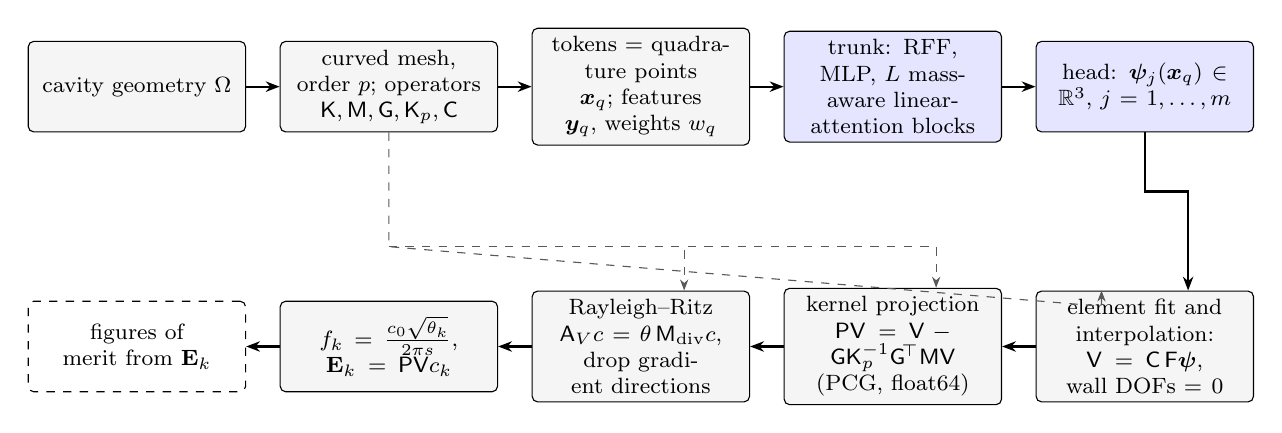
\begin{tikzpicture}[
  font=\footnotesize,
  box/.style={draw, rounded corners=2pt, align=center, text width=2.55cm, minimum height=1.15cm, inner sep=3pt},
  learned/.style={box, fill=blue!10},
  fixed/.style={box, fill=black!4},
  opt/.style={box, dashed},
  arr/.style={-{Stealth[length=5pt]}, thick},
  darr/.style={-{Stealth[length=4pt]}, dashed, gray!70!black}]
  % row 1: geometry -> tokens -> network
  \node[fixed] (geo)  at (0,0)    {cavity geometry $\Omega$};
  \node[fixed] (mesh) at (3.2,0)  {curved mesh, order $p$; operators $\Kmat,\Mmat,\Gmat,\Kp,\Cmat$};
  \node[fixed] (tok)  at (6.4,0)  {tokens $=$ quadrature points $\bm x_q$; features $\bm y_q$, weights $w_q$};
  \node[learned] (trunk) at (9.6,0)  {trunk: RFF, MLP, $L$ mass-aware linear-attention blocks};
  \node[learned] (head)  at (12.8,0) {head: $\bm\psi_j(\bm x_q)\in\R^3$, $j=1,\dots,m$};
  \draw[arr] (geo) -- (mesh);
  \draw[arr] (mesh) -- (tok);
  \draw[arr] (tok) -- (trunk);
  \draw[arr] (trunk) -- (head);
  % row 2: fixed linear algebra layer, right to left
  \node[fixed] (V)   at (12.8,-3.3) {element fit and interpolation: $\Vmat=\Cmat\,\mathsf{F}\bm\psi$, wall DOFs $=0$};
  \node[fixed] (P)   at (9.6,-3.3)  {kernel projection $\Pmat\Vmat=\Vmat-\Gmat\Kp^{-1}\Gmat^{\!\top}\Mmat\Vmat$ (PCG, float64)};
  \node[fixed] (R)   at (6.4,-3.3)  {Rayleigh--Ritz $\Av c=\theta\,\Mdiv c$, drop gradient directions};
  \node[fixed] (out) at (3.2,-3.3)  {$f_k=\tfrac{c_0\sqrt{\theta_k}}{2\pi s}$, $\;\E_k=\Pmat\Vmat c_k$};
  \node[opt]   (qoi) at (0,-3.3)    {figures of merit from $\E_k$};
  \draw[arr] (head.south) -- ++(0,-0.75) coordinate (a) -| ($(V.north)+(0.55,0)$);
  \draw[arr] (V) -- (P);
  \draw[arr] (P) -- (R);
  \draw[arr] (R) -- (out);
  \draw[arr] (out) -- (qoi);
  % operators of the mesh feed the fixed layer
  \draw[darr] (mesh.south) -- ++(0,-1.45) coordinate (b) -- ($(V.north)+(-0.55,1.45-1.65)$) -- ($(V.north)+(-0.55,0)$);
  \draw[darr] (b) -| ($(P.north)+(0.55,0)$);
  \draw[darr] (b) -| ($(R.north)+(0.55,0)$);
\end{tikzpicture}}
\caption{Pipeline of the model. Shaded boxes are learned; grey boxes are fixed linear algebra that depends on the mesh only (the dashed arrows carry the operators of the mesh). The trunk and the head see only points, so the same weights can be run on any conforming space (\cref{rem:04-space}). The figures of merit (dashed box) are evaluated from the predicted fields by the functionals of \cref{sec:formulation} and are not part of the loss in this work. $s$ is the geometry scale.}
\label{fig:pipeline}
\end{figure}

\subsection{Tokens and trunk}\label{sec:04-trunk}

\paragraph{Tokens.}
Let $\mathcal T_h$ be the curved mesh of $\Omega$ with $N_t$ elements and let $\Vh$ be the Nédélec space of order $p$ on it (\cref{sec:formulation}).
On every element we fix the same reference quadrature rule of degree $2p$.
The trunk's tokens are the $N=N_t\,n_q$ quadrature points $\bm x_q$ of all elements, with $n_q=14$ at $p=2$ and $n_q=24$ at $p=3$.
% src: src/data_gen/highorder.py _quadrature (IntegrationRule(TET, 2*order)); n_q = 14, 24 checked with NGSolve 6.2; docs/34 §4.2
Using the quadrature points rather than the mesh vertices matters: coarse curved meshes can have no interior vertex at all, and in a single-sample overfit test the vertex-token variant stalled at a relative eigenvalue error of order $10^{-4}$ whereas quadrature-point tokens reached $10^{-6}$--$10^{-5}$ (\cref{sec:experiments}).
% src: docs/28 §2, §3 (0.8-1.1e-4 and 2.3-3.0e-4 vs 1e-6 - 9e-6)
Each token carries nine features computed on the curved geometry and normalised by the geometry scale: the coordinates $\bm x_q$, the distance to the wall, the unit vector to the nearest wall point, the point volume (quadrature weight, divided by its maximum), and the torsion function $\tau$ ($-\Delta\tau=1$ in $\Omega$, $\tau=0$ on $\partial\Omega$, solved in the $H^1_0$ space of order $p+1$ on the same curved mesh and divided by its maximum).
% src: src/data_gen/highorder.py point_features, wall_features (FEATURE_NAMES_3D: x,y,z, dist, dir x3, volume, torsion); docs/28 §2
The wall features are the only part of the input that sees the boundary; they are computed once per geometry.

\paragraph{Mass-aware linear attention.}
Let $\varphi(\bm\xi)=\sqrt{2/D}\,[\cos(\mathsf B\bm\xi),\sin(\mathsf B\bm\xi)]$ be a random Fourier feature map with a frozen Gaussian matrix $\mathsf B$~\cite{rahimi2007random,tancik2020fourier}, and let $\bm\xi_q$ denote the normalised coordinates.
The embedding is $\bm h^0_q=\mathrm{MLP}([\varphi(\bm\xi_q)\,\Vert\,\bm y_q])$ with the feature vector $\bm y_q\in\R^9$ above.
Each of the $L$ trunk blocks is a pre-norm residual block $\bm h\leftarrow\bm h+\mathrm{Attn}_w(\mathrm{LN}\,\bm h)$, $\bm h\leftarrow\bm h+\mathrm{FFN}(\mathrm{LN}\,\bm h)$, where, per head,
\begin{equation}\label{eq:04-attn}
  [\mathrm{Attn}_w(\bm h)]_i=\frac{\sum_{q} w_q\,\phi(\mathsf Q\bm h_i)^{\!\top}\phi(\mathsf K\bm h_q)\;\mathsf V\bm h_q}{\sum_{q} w_q\,\phi(\mathsf Q\bm h_i)^{\!\top}\phi(\mathsf K\bm h_q)+\varepsilon},\qquad \phi=\mathrm{elu}+1,
\end{equation}
which is the linear attention of Katharopoulos et al.~\cite{katharopoulos2020transformers} with a weight $w_q$ on every key.
The weights are the quadrature weights ($|\det J|$ times the reference weight) normalised to $\sum_q w_q=1$, with $\varepsilon=10^{-6}$.
% src: src/models/layers.py LinearAttention (eps=1e-6), mass_weights; src/data/field_dataset.py (Area = quadrature weights)
Both sums in \eqref{eq:04-attn} are therefore element quadratures of $\int\kappa(\bm h_i,\bm h(\bm y))\,\mathsf V\bm h(\bm y)\,\mathrm d\bm y$ and $\int\kappa(\bm h_i,\bm h(\bm y))\,\mathrm d\bm y$ with a separable kernel $\kappa$, i.e.\ a global integral operator evaluated by the mesh's own quadrature, as in the Galerkin-type attention of Cao~\cite{cao2021choose}.
Refining the mesh changes the sums by quadrature error only, and the evaluation costs $O(N D^2)$ instead of $O(N^2D)$ because $\sum_q w_q\phi(\mathsf K\bm h_q)(\mathsf V\bm h_q)^{\!\top}$ is formed once.
The normalisation $\sum_q w_q=1$ cancels in the ratio except through $\varepsilon$.
The head is a two-layer MLP, $\bm\psi_{1..m}(\bm x_q)=\mathrm{head}([\bm h^L_q\,\Vert\,\varphi(\bm\xi_q)])\in(\R^3)^m$.
Since $\bm\psi_j$ is a function of the point and its features only, it is a geometric vector field: relabelling the mesh does not change it.
Default sizes are $D=128$, $L=4$ blocks, $4$ heads, $m=24$ fields, $K=6$ modes and a 64-dimensional Fourier map with length scale $0.1$ (the small-scale experiments use a reduced configuration, \cref{sec:experiments}).
% src: configs/field_3d.yaml (embed_dim 128, n_layers 4, n_heads 4, n_basis 24, num_field_modes 6, rff_dim 64, rff_length_scale 0.1)

\subsection{From point values to degrees of freedom}\label{sec:04-map}

The point values $\bm\psi_j(\bm x_q)$ are turned into DOFs of $\Vh$ by a fixed linear map in two stages.
\emph{(i) Element fit.}
Let $\mathbb Q_p$ be the space of polynomials of degree $\le p$ in the reference coordinates (dimension $n_\ell=\binom{p+3}{3}$), $\Phi_t\in\R^{n_q\times n_\ell}$ its basis evaluated at the quadrature points of element $t$, and $\mathsf W_t=\mathrm{diag}(|\det J_t(\hat{\bm x}_q)|\,\omega_q)$.
Each Cartesian component of $\bm\psi_j$ is fitted by weighted least squares,
$\bm a_{t,c,j}=\mathsf F_t\,\bm\psi_{t,c,j}$, $\mathsf F_t=(\Phi_t^{\!\top}\mathsf W_t\Phi_t)^{-1}\Phi_t^{\!\top}\mathsf W_t$,
which is exact on $\mathbb Q_p$ because $n_q\ge n_\ell$ ($14\ge10$ at $p=2$, $24\ge20$ at $p=3$).
% src: src/data_gen/highorder.py field_operators (P = solve(A, Phi^T W), W = detJ*wq); n_l = dim P_p = 10, 20 (p+3 choose 3)
\emph{(ii) Interpolation into $\Vh$.}
The discontinuous element-wise polynomial field is mapped to $\Vh$ by a fixed sparse operator $\Cmat$.
In the implementation, $\Cmat$ is the NGSolve conversion operator~\cite{schoeberl2014cpp11} from the vector-valued discontinuous space to $\Vh$: it applies the dual basis of $\Vh$ element by element and averages the DOFs shared between elements.
% src: ngsolve ConvertOperator docstring ("interpolation operator defined by element-wise application of dual shapes (and averaging between elements)"); docs/28 §2 calls it projection-based interpolation
It plays the role of a projection-based interpolation operator~\cite{demkowicz2005projection}; the only properties used below are linearity and element-wise locality.
Zeroing the DOFs on the wall (rows of $\mathsf D_{\rm int}$) enforces $\bm n\times\E=0$ structurally,
\begin{equation}\label{eq:04-V}
  \Vmat_{:,j}=\mathsf D_{\rm int}\,\Cmat\,\mathsf F\,\bm\psi_j,\qquad \Vmat\in\R^{n\times m},
\end{equation}
where $\mathsf F=\mathrm{blockdiag}(\mathsf F_t)$ acts on the stacked point values.
$\Vmat$ is linear in $\bm\psi$, so gradients flow through it by two sparse products.
The operators $\Kmat,\Mmat,\Gmat,\Kp,\Cmat,\mathsf F$ are assembled once per geometry with one explicit integration rule on curved elements, so that the forms used by the model and by the label solver coincide.
% src: AGENTS.md invariants (highorder.volume_measure); docs/28 §2 numerical note

\subsection{Kernel projection}\label{sec:04-proj}

The gradients $\nabla\Sh$ (together with one potential per extra wall component, if the wall has several components) span the kernel of $\Kmat$ on $\Vh$, so a generic $\Vmat$ contains a large spurious gradient part which a Rayleigh quotient would see as $\theta\approx0$.
(In a smoke test of the lowest-order variant about $60\%$ of the mass of the raw basis was gradient.)
% src: docs/20 §6 (grad_frac 0.59, 30 geometries, N0 model)
With $\mathsf B=\Gmat^{\!\top}\Mmat\Vmat$ and $\mathsf Z=\Kp^{-1}\mathsf B$ we define
\begin{equation}\label{eq:04-proj}
  \Pmat\Vmat=\Vmat-\Gmat\mathsf Z,\qquad
  (\Pmat\Vmat)^{\!\top}\Kmat(\Pmat\Vmat)=\Av:=\Vmat^{\!\top}\Kmat\Vmat,\qquad
  \Mdiv:=(\Pmat\Vmat)^{\!\top}\Mmat(\Pmat\Vmat)=\Vmat^{\!\top}\Mmat\Vmat-\mathsf B^{\!\top}\mathsf Z,
\end{equation}
the second identity because $\Kmat\Gmat=0$ and the third because $\Kp\mathsf Z=\mathsf B$ (Schur complement).
$\Pmat\Vmat$ is the $\Mmat$-orthogonal projection of $\Vmat$ onto the discretely divergence-free subspace $W_h=\{\bm v\in\Vh:\bm v^{\!\top}\Mmat\Gmat=0\}$, and neither Gram matrix needs $\Pmat\Vmat$ to be formed.
Here $\Kp=\Gmat^{\!\top}\Mmat\Gmat$ is symmetric positive definite (a PEC cavity has no constant potential), so no zero-mean handling is needed in this E formulation.

$\mathsf Z$ is computed by Jacobi-preconditioned conjugate gradients, batched over samples and over the $m$ right-hand sides, each (sample, column) pair having its own step sizes.
Iteration stops when every column satisfies $\|\mathsf r_j\|_2\le\tau\|\mathsf B_{:,j}\|_2$ with $\tau=10^{-8}$ (checked every ten iterations, at most $3000$ iterations; a warning is raised if the limit is hit).
% src: src/models/hcurl.py _pcg (check_every=10, thr = tol*||rhs||); configs/field_3d.yaml (kp_tol 1e-8, kp_maxiter 3000)
The solve runs in float64.
In float32 the iteration did not converge and $\Mdiv$ was off by about $79\%$ in a test; we attribute this to the cancellation in the Schur complement when $\Vmat$ has a large gradient part.
% src: src/models/hcurl.py project_basis comment ("float32 CG does not converge (M_div off by ~79%, docs/21 B3)"); AGENTS.md invariants
The map $\mathsf B\mapsto\mathsf Z$ is the symmetric linear operator $\Kp^{-1}$, so the backward pass is one more solve with the same matrix, $\bar{\mathsf B}=\Kp^{-1}\bar{\mathsf Z}$; we implement this as a custom autograd function in PyTorch~\cite{paszke2019pytorch} rather than differentiating through the iterations.
% src: src/models/hcurl.py KpSolve

\subsection{Rank-revealing Rayleigh--Ritz layer}\label{sec:04-ritz}

The Ritz problem on $\spn(\Pmat\Vmat)$ is $\Av\,c=\theta\,\Mdiv\,c$.
It is degenerate exactly when a combination $\Vmat c$ is a pure gradient: then $\Pmat\Vmat c=0$ and both $\Mdiv c$ and $\Av c$ vanish.
A ridge would assign such directions an arbitrary $\theta$ inside the spectrum, and the losses of \cref{sec:04-loss} never see gradient content, so training would not push them away.
We therefore reveal the rank first.
Let $\mathsf D=\mathrm{diag}(\Vmat^{\!\top}\Mmat\Vmat)^{-1/2}$ and $\mathsf D(\Vmat^{\!\top}\Mmat\Vmat)\mathsf D+\epsilon\mathsf I=\mathsf L\mathsf L^{\!\top}$ ($\epsilon=10^{-8}$).
The eigenvalues $\mu_i\in[0,1]$ of $\mathsf L^{-1}\mathsf D\Mdiv\mathsf D\mathsf L^{-\top}=\mathsf Q\,\mathrm{diag}(\mu)\mathsf Q^{\!\top}$ are the divergence-free mass fractions of the whitened directions.
Directions with $\mu_i\le\tau_{\rm drop}=10^{-6}$ are discarded; with the remaining ones, $\mathsf W=\mathsf L^{-\top}\mathsf Q_{\rm kept}\,\mu_{\rm kept}^{-1/2}$ and
\begin{equation}\label{eq:04-ritz}
  \mathsf W^{\!\top}\mathsf D\,\Av\,\mathsf D\mathsf W\,\mathsf y=\theta\,\mathsf y,\qquad c=\mathsf D\mathsf W\mathsf y,
\end{equation}
a standard symmetric eigenproblem of size $r'\le m$.
% src: src/models/hcurl.py projected_eigh (mass_ridge 1e-8, drop_tol 1e-6); docs/20 §2
Discarded directions receive $\theta=+\infty$ (implemented as a large finite number) and sort last.
The $K$ smallest values give the predicted frequencies $f_k=c_0\sqrt{\theta_k}/(2\pi s)$, where $s$ is the geometry scale of the normalised coordinates (eigenvalues scale as $s^{-2}$), and the fields $\E_k=\Pmat\Vmat c_k$, which are $\Mmat$-orthonormal by construction.
Both symmetric eigendecompositions use a custom backward pass in which the factor $1/(\lambda_j-\lambda_i)$ of the standard eigenvector gradient~\cite{ionescu2015matrix,seeger2017autodiff} is replaced by the Lorentzian-broadened $\Delta/(\Delta^2+\varepsilon_{\rm b})$, $\varepsilon_{\rm b}=10^{-4}$.
Without this the gradient is infinite for the (near-)degenerate pairs that are the normal case in cavities (dipole and quadrupole pairs).
% src: src/models/layers.py BroadenedEigh; configs/field_3d.yaml (eig_broadening 1e-4)

\subsection{Upper-bound guarantee}\label{sec:04-bound}

Let $n_{\rm f}$ be the number of free (non-wall) DOFs, and denote by $\lamh_1\le\lamh_2\le\dots$ the positive eigenvalues of $\Kmat x=\lambda\Mmat x$ on $\Vh$ with the wall DOFs removed; the frequencies are the monotone image $f=c_0\sqrt{\lambda}/(2\pi s)$, so everything below holds for $\lambda$ and for $f$ alike.
We use one standing assumption on the space.
\begin{description}
\item[(A)] The columns of $\Gmat$ span $\ker\Kmat$ on $\Vh$, and $\Mmat$ is positive definite.
\end{description}
(A) is the exactness of the discrete sequence $\Sh\xrightarrow{\nabla}\Vh\xrightarrow{\curl}$ for the conforming spaces used here, with one extra wall potential per additional connected component of $\partial\Omega$~\cite{hiptmair2002finite,arnold2006finite}.
Under (A), $\Vh=\ker\Kmat\oplus W_h$ is an $\Mmat$-orthogonal splitting and $\Kmat$ is positive definite on $W_h$.
Moreover the positive eigenvalues of the full problem are exactly the eigenvalues of the pencil restricted to $W_h$: if $\Kmat x=\lambda\Mmat x$ with $\lambda>0$ then $\bm g^{\!\top}\Mmat x=\lambda^{-1}\bm g^{\!\top}\Kmat x=0$ for every $\bm g\in\ker\Kmat$, so $x\in W_h$; counting dimensions gives the claim.
Courant--Fischer~\cite{parlett1998symmetric} therefore reads
\begin{equation}\label{eq:04-minmax}
  \lamh_k=\min_{\substack{S\subset W_h\\ \dim S=k}}\ \max_{0\ne\bm v\in S}\frac{\bm v^{\!\top}\Kmat\bm v}{\bm v^{\!\top}\Mmat\bm v}.
\end{equation}

\begin{proposition}[Ritz values are upper bounds]\label{prop:upper-bound}
Assume (A) and that $\mathsf Z$ is the exact solution of $\Kp\mathsf Z=\mathsf B$.
Let $\Vmat\in\R^{n\times m}$ be arbitrary (with zero wall rows) and let $r'$ be the number of directions kept by the Ritz layer of \cref{sec:04-ritz}.
Then $r'=\dim U'$ for a subspace $U'\subset\spn(\Pmat\Vmat)\subset W_h$, the $r'$ finite outputs $\theta_1\le\dots\le\theta_{r'}$ of \eqref{eq:04-ritz} are the Rayleigh--Ritz values of $(\Kmat,\Mmat)$ on $U'$, and
\[
  \theta_k\ \ge\ \lamh_k\ >\ 0\qquad(k=1,\dots,r'),
\]
while $\theta_k=+\infty$ for $k>r'$.
In particular no spurious zero mode occurs, and $f_k^{\rm pred}\ge f_{h,k}$ for every network weight, for every input geometry, and before as well as after training.
\end{proposition}

\begin{proof}
\emph{Step 1: $\Pmat\Vmat$ lies in $W_h$.}
$\Gmat^{\!\top}\Mmat\Pmat\Vmat=\mathsf B-\Kp\mathsf Z=0$, so every column of $\Pmat\Vmat$ is $\Mmat$-orthogonal to $\ker\Kmat=\mathrm{range}\,\Gmat$ by (A).

\emph{Step 2: the Ritz layer computes Rayleigh--Ritz values on $U'$.}
By construction $\mathsf W^{\!\top}\mathsf D\Mdiv\mathsf D\mathsf W=\mathsf I_{r'}$: the ridge $\epsilon$ enters only $\mathsf L$ and cancels in the normalisation $\mathsf W^{\!\top}\mathsf D\Mdiv\mathsf D\mathsf W=\mu_{\rm kept}^{-1/2}\mathsf Q_{\rm kept}^{\!\top}(\mathsf L^{-1}\mathsf D\Mdiv\mathsf D\mathsf L^{-\top})\mathsf Q_{\rm kept}\mu_{\rm kept}^{-1/2}$.
Put $\mathsf Y=\mathsf D\mathsf W\in\R^{m\times r'}$.
Then $(\Pmat\Vmat\mathsf Y)^{\!\top}\Mmat(\Pmat\Vmat\mathsf Y)=\mathsf Y^{\!\top}\Mdiv\mathsf Y=\mathsf I$ by \eqref{eq:04-proj}, so the columns of $\Pmat\Vmat\mathsf Y$ are $\Mmat$-orthonormal (in particular linearly independent) and span a subspace $U'\subset\spn(\Pmat\Vmat)$ of dimension $r'$.
The matrix in \eqref{eq:04-ritz} equals $\mathsf Y^{\!\top}\Av\mathsf Y=(\Pmat\Vmat\mathsf Y)^{\!\top}\Kmat(\Pmat\Vmat\mathsf Y)$, the Gram matrix of $\Kmat$ in an $\Mmat$-orthonormal basis of $U'$; its eigenvalues are by definition the Rayleigh--Ritz values of $(\Kmat,\Mmat)$ on $U'$~\cite{parlett1998symmetric}, and by Courant--Fischer on $U'$
\[
  \theta_k=\min_{\substack{S\subset U'\\ \dim S=k}}\ \max_{0\ne\bm v\in S}\frac{\bm v^{\!\top}\Kmat\bm v}{\bm v^{\!\top}\Mmat\bm v}.
\]
The $m-r'$ discarded directions contribute only the placeholder value.

\emph{Step 3: comparison.}
$U'\subset W_h$ by Step~1, so the minimum defining $\theta_k$ runs over a subfamily of the $k$-dimensional subspaces in \eqref{eq:04-minmax}, hence $\theta_k\ge\lamh_k$.
Positivity follows from $\lamh_1>0$, which is (A).
\end{proof}

The statement is about the \emph{discrete} eigenvalues of the space the model is run in.
Since $\Vh\subset H_0(\curl;\Omega)$ is a conforming space with the exactness property (A), $\lamh_k\to\lambda_k$ as $h\to0$ or $p\to\infty$ (discrete compactness~\cite{boffi2010finite}), but $\theta_k\ge\lamh_k$ does not by itself imply $\theta_k\ge\lambda_k$, and we make no such claim for the exact eigenvalue.
In our data the discrete eigenvalues of the order-two model space exceeded those of the order-three label space in every comparison ($+0.004$ to $+0.047\,\%$ in frequency).
% src: docs/34 §8.1 (frequency LF/HF - 1 = +0.004 ... +0.047 %)
Two further consequences are used by the losses.
First, $\sum_{i\le m}\theta_i^{-1}\le\sum_{i\le m}\lamh_i^{-1}$ when $\Pmat\Vmat$ has full column rank, with equality iff $\spn(\Pmat\Vmat)$ is the span of the $m$ lowest eigenvectors; the left side is $\mathrm{tr}(\Av^{-1}\Mdiv)$.
Second, the bound is attained from above as the basis improves: $\theta_k-\lamh_k$ is non-negative and shrinks with the best-approximation error of the eigenvectors in $\spn(\Pmat\Vmat)$ in the energy norm~\cite{boffi2010finite}.

\begin{remark}[Inexact projection]\label{rem:04-inexact}
The proposition is exact only if $\Kp\mathsf Z=\mathsf B$ holds exactly; the CG solve leaves a residual $\rho=\Kp\tilde{\mathsf Z}-\mathsf B$ with $\|\rho_{:,j}\|\le\tau\|\mathsf B_{:,j}\|$, $\tilde{\mathsf Z}=\mathsf Z+\delta$.
Two things happen.
\emph{The numerator is unaffected.} $\Av=\Vmat^{\!\top}\Kmat\Vmat$ is evaluated directly and $\Kmat\Gmat=0$, so the curl energy of the computed field $\tilde{\Pmat}\Vmat=\Pmat\Vmat-\Gmat\delta$ is that of the exact projection: the residual gradient component carries no curl energy.
\emph{The denominator is perturbed.} The layer uses $\tilde{\mathsf M}_{\rm div}=\Vmat^{\!\top}\Mmat\Vmat-\mathsf B^{\!\top}\tilde{\mathsf Z}=\Mdiv+\mathsf E$ with $\mathsf E=-\mathrm{sym}(\mathsf Z^{\!\top}\rho)$.
For a coefficient vector $c$, $c^{\!\top}\mathsf Ec=-\langle\Gmat\mathsf Zc,\Gmat\delta c\rangle_{\Mmat}$ and $\Gmat\mathsf Zc$ is the $\Mmat$-projection of $\Vmat c$ onto $\mathrm{range}\,\Gmat$, so
\[
  |c^{\!\top}\mathsf Ec|\le\|\Vmat c\|_{\Mmat}\,\|\rho c\|_{\Kp^{-1}},\qquad
  \eta(c):=\frac{|c^{\!\top}\mathsf Ec|}{c^{\!\top}\Mdiv c}\le\frac{\|\rho c\|_{\Kp^{-1}}}{\mu(c)\,\|\Vmat c\|_{\Mmat}},\quad
  \mu(c)=\frac{\|\Pmat\Vmat c\|_{\Mmat}^2}{\|\Vmat c\|_{\Mmat}^2}.
\]
If $\bar\eta=\sup\eta(c)<1$ over the kept coefficient subspace, every computed Rayleigh quotient is at least $(1+\bar\eta)^{-1}$ times the Rayleigh quotient of the exact field $\Pmat\Vmat c\in W_h$, and the same min--max argument gives
\[
  \tilde\theta_k\ \ge\ \lamh_k/(1+\bar\eta).
\]
So an inexact solve can lower the Ritz values only by a relative amount $\bar\eta$, which is proportional to the CG residual and inversely proportional to the divergence-free fraction $\mu(c)$; this is why directions with $\mu\le\tau_{\rm drop}$ are discarded rather than ridged.
The field actually returned, $\tilde{\Pmat}\Vmat c$, has the same numerator and the larger mass $c^{\!\top}\Mdiv c+\|\Gmat\delta c\|_{\Mmat}^2$, so its own Rayleigh quotient is also lowered by at most $O(\bar\eta)$.
We do not bound $\bar\eta$ a priori; the bound $\theta_k\ge\lamh_k$ is therefore a rigorous statement for exact arithmetic and an observed one for the implemented solver, and it was checked on all evaluated predictions: all Ritz values exceeded the discrete eigenvalue of the evaluated space, with smallest margins of $+0.006\,\%$ (native space), $+0.009\,\%$ (order three and refined mesh) and $+0.47\,\%$ (equal-cost study).
% src: docs/34 §4.1 (min. diff +0.006 %), §4.2 (min. +0.009 %), §8.2 (at least +0.47 %)
Floating-point rounding in the Gram matrices is not covered by the argument.
\end{remark}

\begin{remark}[Space independence]\label{rem:04-space}
The network sees only points, their features and their quadrature weights; the Ritz layer needs only $\Kmat,\Mmat,\Gmat,\Kp$ and the fixed maps $\Cmat,\mathsf F$ of the space in which it is evaluated.
Nothing in \cref{prop:upper-bound} depends on how $\Vmat$ was produced, so the same trained weights can be evaluated on another conforming space (order three on the same mesh, or a uniformly refined mesh) by rebuilding these operators; the Ritz values are then upper bounds of the discrete eigenvalues of \emph{that} space.
This was measured in \cref{sec:experiments}; the bound held in every case (margin $\ge+0.009\,\%$).
% src: docs/34 §4.2
The accuracy does not improve in the larger space, because the learned fields $\bm\psi_j$ are the same smooth fields and the token density and the point-volume feature differ from training ($14$ versus $24$ points per element).
% src: docs/34 §4.2 (Doğruluk iyileşmiyor; p3 24 vs p2 14 points per tet)
\end{remark}

\subsection{Losses}\label{sec:04-loss}

Let $\mathsf T=[t_1,\dots,t_n]$ be the stored target fields (the $n$ lowest label eigenvectors projected onto $\Vh$, \cref{sec:data}), which are discretely divergence-free.
For $\mathsf N\in\{\Mmat,\Kmat\}$ let $\mathsf G_{\mathsf N}$ be the Gram matrix of $[\Pmat\Vmat\,|\,\mathsf T]$ in the $\mathsf N$-inner product.
It is obtained without forming $\Pmat\Vmat$ and with the same $\mathsf Z$ (no second CG solve): the $\Pmat\Vmat$ block is $\Mdiv$ or $\Av$, the cross blocks are $\Vmat^{\!\top}\Mmat\mathsf T-\mathsf Z^{\!\top}(\Gmat^{\!\top}\Mmat\mathsf T)$ and $\Vmat^{\!\top}\Kmat\mathsf T$.

\paragraph{Span loss.}
The fraction of target $t_k$ not captured by $\spn(\Pmat\Vmat)$ in the $\mathsf N$-norm is
\[
  r_k^{\mathsf N}=1-\frac{\|\Pi_{\mathsf N}t_k\|_{\mathsf N}^2}{\|t_k\|_{\mathsf N}^2}\in[0,1],
\]
with $\Pi_{\mathsf N}$ the $\mathsf N$-orthogonal projector onto $\spn(\Pmat\Vmat)$, evaluated by a Cholesky solve of the Jacobi-scaled Gram with a relative ridge of $10^{-9}$.
The span loss is
\begin{equation}\label{eq:04-span}
  \mathcal L_{\rm span}=\frac1n\sum_{k=1}^n\sqrt{\tfrac12\big(r_k^{\Mmat}+r_k^{\Kmat}\big)+10^{-8}}.
\end{equation}
% src: src/training/lightning_module.py span_residual, _span_terms (span_norm both, span_root true, span_ridge 1e-9, eps 1e-8)
$\sqrt{r_k^{\Mmat}}$ is the relative best-approximation error of $t_k$ in $L^2$, and $\sqrt{r_k^{\Kmat}}$ the one in the energy norm, which controls the Ritz eigenvalue error; the square-root form keeps the gradient from vanishing as the span becomes accurate.
$\mathcal L_{\rm span}$ is invariant under any invertible recombination of the columns of $\Vmat$ and under sign changes and rotations inside degenerate target clusters, so no eigenvalue matching or cluster detection is needed.

\paragraph{Self-supervised term.}
$\mathcal L_{\rm ss}=-\log\mathrm{tr}(\Av^{-1}\Mdiv)=-\log\sum_i\theta_i^{-1}$, evaluated by a Cholesky solve.
It needs no labels and, by the consequence of \cref{prop:upper-bound} above, is bounded and minimised exactly when the span is the lowest-$m$ eigenspace.
Because $\Mdiv$ is the projected mass, a nearly-gradient column cannot lower it.
For comparison, the unprojected compliance was measured to blow up by more than a factor $10^3$ in such a case.
% src: docs/20 §3 (selfsup: "Neredeyse-gradyan bir kolonda projeksiyonsuz compliance >10^3x patlar (test edildi)")

\paragraph{Conditioning term.}
$\mathcal L_{\rm ortho}=\frac{1}{m(m-1)}\sum_{i\ne j}\big(\Mdiv_{ij}\big)^2/(\Mdiv_{ii}\Mdiv_{jj})$ penalises the collinearity of the learned fields (mean squared off-diagonal mass correlation) and keeps $\spn(\Pmat\Vmat)$ well conditioned.

\paragraph{Frequency term.}
$\mathcal L_{\rm freq}=\frac1K\sum_{k=1}^K(z_k-z_k^\star)^2$, where $z=(f-\bar f)/\sigma_f$ are frequencies in GHz standardised with the mean and standard deviation of the training labels.
Gradients reach the network through both eigendecompositions of \cref{sec:04-ritz}.

\paragraph{Total and fidelity weights.}
$\mathcal L=\lambda_{\rm span}\mathcal L_{\rm span}+\lambda_{\rm ss}\mathcal L_{\rm ss}+\lambda_{\rm ortho}\mathcal L_{\rm ortho}+\lambda_{\rm freq}\mathcal L_{\rm freq}$ with defaults $(1,\,0.01,\,0.01,\,0.1)$.
% src: configs/field_3d.yaml (span_weight 1.0, selfsup_weight 0.01, ortho_weight 0.01, freq_weight 0.1)
A loss on the figures of merit exists in the code but is disabled for this model.
Every training sample carries a label fidelity $\mathrm{fid}\in\{\LF,\HF\}$ (\cref{sec:multifidelity}); the span and frequency terms of sample $b$ are multiplied by $\omega_{\mathrm{fid}(b)}$, and the frequency term additionally by $s_{\mathrm{fid}(b)}$, so the batch loss is the sample mean of $\omega_{\mathrm{fid}(b)}\ell_b$ for the span part and of $\omega_{\mathrm{fid}(b)}s_{\mathrm{fid}(b)}\ell_b$ for the frequency part.
The scale $s_{\HF}$ exists because $\HF$ frequencies can lie below the lowest value the order-two Ritz layer can reach, whereas $\LF$ frequencies are exactly the discrete eigenvalues of the model space itself and are reachable by the Ritz values.
The defaults are $\omega=(1,1)$ and $s=(1,1)$, i.e.\ no reweighting.
% src: docs/34 §2, configs/field_3d.yaml (fidelity_weights, fidelity_freq_scale), src/training/lightning_module.py _compute_loss_3d

\subsection{Cost}\label{sec:04-cost}

Per geometry the trunk costs $O(ND^2L)$ time and $O(ND)$ memory, which is linear in the number of tokens $N=n_qN_t$; with gradient checkpointing (recomputing the encoder and each attention and feed-forward half in the backward pass) the peak training memory of a run fell from $9.9$ to $3.8$\,GB with bit-identical gradients.
% src: docs/28 §4 (training memory: 9.9 GB -> 3.8 GB, gradients bit-identical)
The mesh-dependent part dominates.
The vector $\Vmat$ has $nm$ entries, and each CG iteration costs $O(\mathrm{nnz}(\Kp)\,m)$ in float64; the number of iterations grows roughly like $h^{-1}$ (in the lowest-order variant: from $60$ to $170$ iterations while the edge count grows from $2\,053$ to $47\,919$), and the backward pass adds one more solve.
% src: docs/20 §5 (PCG iterations 60 ... 170 for N_e 2053 ... 47919)
The Ritz layer is negligible: it handles $m\times m$ matrices.
Mesh size is therefore the critical parameter.
On a curved pillbox-with-pipes mesh of $10.5$k tetrahedra, order two has $112$k DOFs, $41$k potentials and $148$k tokens, and order three $282$k DOFs, $100$k potentials and $253$k tokens, with operator assembly of $7$--$10$\,s and $37$\,s on one thread ($25$M and $105$M non-zeros in $\Kmat,\Mmat,\Gmat,\Kp,\Cmat$).
% src: docs/28 §4 table (netgen curvaturesafety 2: 10.5k tets, p2 112k/41k/148k/25M/7-10 s; p3 282k/100k/253k/105M/37 s)
For a mesh of $13$k tetrahedra ($183$k tokens, order two) on four CPU threads we measured $4.2$\,s for operator assembly, $0.34$\,s for batch collation and about $22$\,s per training step.
% src: docs/28 §4 "Measured per step" (13k tets, 183k tokens, CPU, 4 threads)
The operators are rebuilt per sample rather than stored, since storing them would take about $0.4$\,GB per sample at order two, whereas the curved mesh itself is $1.4$\,MB.
% src: docs/28 §4 Storage (1.4 MB per sample; ~0.4 GB per sample at p2)
Order three is therefore impractical for training on a CPU, which is one motivation for the low-fidelity labels of \cref{sec:multifidelity}.

\section{Dataset generation}\label{sec:data}

A parametric generator draws a CAD solid; a curved tetrahedral mesh is built on it; the lowest $\nmodes$ modes are computed in $H(\mathrm{curl})$ of order three with adaptive remeshing (high-fidelity labels, $\HF$); and the fields are projected onto the order-two space of a smaller model mesh on which the network operates.
Geometry is built with OpenCascade~\cite{opencascade} through gmsh~\cite{geuzaine2009gmsh}; meshing, curving and all finite-element solves use Netgen~\cite{schoberl1997netgen} and NGSolve~\cite{schoberl2014cpp11}.
The eigenproblem is the closed-cavity problem of \cref{sec:formulation} in the $\E$ formulation, which admits cavities with handles and floating conductors; beam pipes are capped by flat PEC walls.
% src: AGENTS.md invariants (E formulation only); docs/19 §6.1; docs/19 §2 (pipes capped)

\subsection{Geometry families}\label{sec:05-geometry}

Eight families with CAD solids are used for field labels (\cref{tab:05-families}).
A free-form family exists only for the lowest-order data path (no CAD solid), and five further families (plain box, quarter-wave coaxial, pillbox with side ports, 6--9-cell elliptical chains, junction boxes) are held out of distribution.
The controlled experiments of \cref{sec:experiments} use one family (pillbox cells with pipes).
% src: dataset_generator_3d.py FAMILIES, parse_args (discrete families dropped for labels=field); cavity_shapes.OOD_FAMILIES; BRIEF §1
Parameters are drawn uniformly; with Sobol' sampling the first 64 draws of sample $i$ (family and shape parameters) come from the $i$-th point of one scrambled Sobol' sequence~\cite{sobol1967distribution,virtanen2020scipy}, later re-draws from a pseudo-random stream.
An optional smooth random deformation of the mesh nodes (3--8 sinusoidal waves, Lipschitz constant below one so that the map stays injective) is available and switched off in our experiments.
% src: dataset_generator_3d.py _sample_rng (qmc.Sobol d=64, scramble=True); docs/19 §2 (deformation); docs/34 §3 (--deform_prob 0)

\begin{table}[t]
\centering
\caption{Families with CAD solids used for field labels: main parameters (uniform ranges, $\beta$ = relative cell length). Corner radii obey the fillet floor.}
\label{tab:05-families}
\small
\begin{tabular}{@{}l p{0.78\linewidth}@{}}
\toprule
Family & Main parameters \\
\midrule
elliptical & 1--5 cells; $R_{eq}\in[40,110]$\,mm, $R_{iris}/R_{eq}\in[0.25,0.42]$, $L/R_{eq}\in[0.45,0.65]\beta$, $A/L\in[0.6,0.9]$, $B/A\in[0.6,1.3]$, $a/L\in[0.12,0.35]$, $b/a\in[0.65,1.9]$; $\beta<1$ in 25\,\%, TESLA/LL/ICHIRO anchors in 30\,\%, port stubs in 35\,\% \\
re-entrant & $R\in[30,70]$\,mm, $L_c/R\in[0.4,1.6]$, $r_p/R\in[0.10,0.25]$, nose gap $g/L_c\in[0.15,0.75]$, cone angle $-25^\circ\ldots35^\circ$ \\
pillbox, pipes & $R\in[30,60]$\,mm, $L_c/R\in[0.4,1.6]$, $r_p/R\in[0.12,0.35]$ \\
ridged box & $a\in[40,100]$, $b\in[30,80]$, $d\in[20,60]$\,mm; 1--2 ridges; optional beam pipes \\
composite & cylinder or ellipsoid body ($R_0\in[25,50]$\,mm), 1--4 attached primitives, 0--2 dents \\
half-wave coaxial & $R_o\in[30,60]$, $L\in[80,200]$\,mm, $r_i/R_o\in[0.2,0.5]$; optional taper and transverse port \\
spoke & tank $R_t\in[50,100]$\,mm, 1--2 spokes, optional beam bore \\
drift-tube linac & tank $R_t\in[50,100]$\,mm, $L_c/R_t\in[0.5,0.9]$, 1--3 drift tubes on stems \\
\bottomrule
\end{tabular}
% src: cavity_shapes.py draw_elliptical, _draw_half, build_reentrant, build_pillbox_pipes, build_ridged_box, build_composite, build_hwr, build_spoke, build_dtl; docs/19 §2
\end{table}

\paragraph{Elliptical half-cells.}
A half-cell joins an iris ellipse $(a,b)$ and an equator ellipse $(A,B)$ by their common tangent line (least-squares solve, five starting points, tolerance $10^{-15}$).
A wall is accepted if the radius does not decrease along it and, for a re-entrant wall, its angle to the beam axis is at most $105^\circ$ and it stays at least $0.05\,R_{eq}$ from the iris plane.
End half-cells differ from the mid-cell with probability $0.6$ (e.g.\ iris radius $\times[1,1.35]$, $a,b\times[0.5,1.05]$).
Published designs enter as sampling centres only (perturbed by $\pm10\,\%$ and rescaled); labels always come from the finite-element solve.
The ranges were widened until all $14$ published reference half-cells that we compiled were accepted: the TESLA mid-cell and both end cups~\cite{aune2000superconducting}, the low-loss and ICHIRO cells~\cite{juntong2009highgradient}, NLSF and NLSF-RE, the Cornell ERL mid-cell and both ends, FCC-ee C3794, C3795 (mid and end) and FCCUROS5.
Four of them were rejected by the earlier solver tolerance and overlap rule.
Several of these dimensions could not be checked against full texts, so we treat them as plausible reference shapes, not as authoritative design data.
Of random $\beta=1$ mid-cells, \SI{65.1}{\percent} are accepted (\SI{50}{\percent} with the earlier rules); rejected draws are replaced, so no sample is lost but the distribution is truncated.
% src: docs/33 §12 "Ölçülenler" (14 half-cells accepted, four rejected before; 65.1 % vs 50 %); docs/33 §11 (full texts unavailable, some dimensions only from an open-source design code); cavity_shapes.py half_cell_wall, END_CELL_RANGES, MAX_WALL_ANGLE, WEB_MIN

\paragraph{Fillet floor.}
A corner radius far below the cavity size forces a curved mesh into many tiny elements (netgen sizes an element on a curved face as about radius over curvature safety) while changing frequencies little.
Every drawn corner radius is therefore raised to at least $0.05$ times the cavity size (never above the builder's feasible maximum), and re-entrant edges left by boolean operations (port, bore and pipe junctions) are rounded with the same rule; where this fails the solid keeps its sharp edges and its surface peaks are stored as NaN.
For pillbox cells with pipes ($R=\SI{57}{mm}$, $r_p=\SI{17}{mm}$) floors of $0.02$, $0.04$, $0.06$, $0.08$ (iris radius \SI{1.2}{mm}--\SI{4.5}{mm}) give $45$k, $30$k, $25$k and $18$k tets.
Small fillets thus drive the element count: four draws of the ridged box, which has fillets along every edge, gave $38$k--$89$k tets, four draws of the spoke family $5.2$k--$7.8$k (curvature safety 2, before adaptive refinement).
% src: dataset_generator_3d.py min_fillet default 0.05 (labels=field); docs/29 §2.1 table and §2.4; docs/30 §3 (rounding, NaN peaks)

\subsection{Curved meshes}\label{sec:05-mesh}

Netgen generates tetrahedra (curvature safety $2$, grading $0.5$) and bends them onto the CAD surfaces to geometry order three.
The element quality is the ratio of the minimum to the maximum Jacobian determinant over each element's integration points ($\le0$: folded).
Frequencies hardly depend on it, wall quantities strongly: on one pillbox cell with pipes (8\,\% fillet floor) a mesh with 9k tets and a minimum ratio of $0.010$ gave frequencies within $10^{-5}$ but $\Qz$ off by $50\,\%$ and surface peaks off by $100$--$1600\times$; at 16k tets and ratio $0.069$ the errors were $10^{-6}$ in frequency and $2\cdot10^{-6}$ in $\Qz$ (reference: the locally repaired 18k-tet mesh, ratio $0.35$); a mesh at curvature safety $1$ folded.
% src: docs/29 §2.2 table

Meshes are accepted at a ratio of at least $0.05$; elements below $0.1$ are bisected and re-curved (three passes, about $+5\,\%$ tets), and only if that fails the mesh is regenerated with doubled curvature safety (about $3\times$ the tets).
Draws with more than $30\,000$ tets are rejected and re-drawn.
% src: docs/29 §2.2 (defaults, thresholds, repair), §2.3 (healing), field_labels.py DEFAULTS max_elements 30000


\subsection{Adaptive order-three labels}\label{sec:05-adaptive}

On each mesh the $\nmodes$ lowest modes (plus one) are computed in $H_0(\mathrm{curl})$ of order three by shift-invert Arnoldi iteration~\cite{lehoucq1998arpack} with the kernel projection after every solve; modes have unit $L^2$ norm, so $\int|\curl\E_k|^2=\lambda_k$.
With $\mathcal R$ the averaging interpolation into the continuous vector Lagrange space of the same order, the jumps of the discrete fields serve as error indicator, in the spirit of recovery estimators~\cite{zienkiewicz1987simple}:
\begin{align*}
\eta_{\mathrm{vol},T}^2 &= \sum_{k=1}^{\nmodes}\frac{\|\curl\E_k-\mathcal R\curl\E_k\|_T^2+\lambda_k\|\E_k-\mathcal R\E_k\|_T^2}{\lambda_k},\\
\eta_{\mathrm{wall},T}^2 &= \sum_{k=1}^{\nmodes}\Bigl(\frac{\int_{\partial T\cap\bdry}|\curl\E_k-\mathcal R\curl\E_k|^2}{\int_{\bdry}|\curl\E_k|^2}+\frac{\int_{\partial T\cap\bdry}|\E_k-\mathcal R\E_k|^2}{\int_{\bdry}|\E_k|^2}\Bigr).
\end{align*}
% src: docs/30 §2; adaptive.py indicator
The volume term estimates the relative eigenvalue error, which is second order in the field error.
Wall loss and surface peaks are first order in the field error at the wall, hence the separately normalised wall term; at the accuracy targets both terms are of order $10^{-6}$ and are added with equal weight.
% src: docs/30 §2

\paragraph{Remeshing instead of bisection.}
Bisection of marked elements on curvature-graded meshes has a closure that explodes: marking 200 of 8109 tets of a pillbox cell with pipes produced $29$k tets ($105$ new per marked tet).
Each iteration therefore builds a new mesh from an error-equidistributing size field,
$h_{\mathrm{new},T}=h_T\bigl(\rho\,\overline{\eta^2}/\eta_T^2\bigr)^{1/(2p)}$ with $\eta_T^2=\eta_{\mathrm{vol},T}^2+\eta_{\mathrm{wall},T}^2$, $\rho=0.25$, $h_{\mathrm{new}}/h\in[0.3,1]$ and $p$ the polynomial order, passed to Netgen as local size restrictions at the element centroids.
The restrictions accumulate over iterations (rebuilding from the latest field alone oscillates); the predicted element count matched Netgen's within $15\,\%$ and is scaled down uniformly if it exceeds the DOF budget.
The start mesh is coarse (curvature safety $1.5$, falling back to $2$ if elements fold).
% src: docs/30 §4; adaptive.py mesh_remesher, size_field

\paragraph{Stopping.}
Refinement stops when, between two consecutive levels (at least two solves), the relative change of the cluster-mean frequency is below $10^{-6}$ and the relative changes of cluster-mean $\Qz$ and $G$, summed $\RoQ$ (clusters with $\RoQ$ above $1\,\%$ of the largest) and maximum $\Epk$, $\Bpk$ are below $10^{-3}$; near-degenerate modes (spacing $<10^{-3}$) are grouped so the test does not depend on the rotation inside a pair.
Otherwise it stops when the next mesh would exceed the DOF budget (default 900k label DOFs, about \SI{12}{GB}) or after eight levels; peaks are left out for samples with sharp edges.
The criterion compares successive levels and is not an error bound; the targets (frequency $10^{-5}$, $\Qz$, $G$, $\RoQ$ $0.2\,\%$, peaks $1\,\%$) are checked against closed forms in \cref{sec:05-validation}.
A budget can bind early: in our controlled experiments the 150k-DOF budget was exhausted after the first order-three solve, so the high-fidelity label there is one order-three solve on the start mesh.
% src: docs/30 §1, §6; adaptive.py DEFAULTS, invariant_qoi, adaptive_modes; docs/34 §3 (adapt_iters = 1, adapt_stop = budget)

\subsection{Label mesh, model mesh and storage}\label{sec:05-transfer}

The \emph{label mesh} is the finest adaptive level and supplies frequencies, figures of merit and the order-three fields.
The \emph{model mesh} is the finest level with at most $10\,000$ tets (about $10^5$ order-two DOFs per geometry); if the start mesh already exceeds this it is the model mesh, and if the final mesh fits both coincide.
% src: docs/30 §5, §6 (model_max_elements 10000, about 100k DOF)
On one mesh the order-two space is nested in the order-three space, so the $L^2$ projection is the exact best approximation; on a coarser model mesh the label fields are evaluated at the model mesh's $216$ integration points per tet (located once for all modes) and projected, $\mathsf M_2\mathsf u_2=\int\mathbf v_2\cdot\E_3$.
We store, per mode, $\text{proj\_err}=\|\E_3-\E_2\|/\|\E_3\|$ and the Rayleigh quotient of $\E_2$ in the model space.
On two pillbox-with-pipes model meshes $\text{proj\_err}$ was $0.18$--$0.54\,\%$ and the Rayleigh quotients exceeded the order-three frequencies by $0.04$--$0.9\,\%$, a floor that a Ritz layer in this space cannot go below.
% src: docs/30 §5 (proj_err 1.8e-3–5.4e-3; p2 floor 4e-4–8.6e-3 on meshes of 11300 and 13052 tets), docs/31 §1

Each geometry is stored as the Netgen mesh file of the model mesh, the BREP of the meshed shape, the frequencies, the projected fields (single precision, wall rows zero), the figures of merit, the axial field, and the wall-distance token features of \cref{sec:method}; about \SI{9}{MB} for ten modes.
% src: docs/29 §1, §4
Mesh generation is not bit-reproducible, so the stored mesh is the record of a sample.
A mesh repaired by bisection keeps a refinement hierarchy whose DOF numbering differs from that of the saved-and-reloaded mesh (in one case $116\,322$ vs.\ $115\,704$ order-two DOFs).
Meshes are therefore rebuilt through a file round trip before storage; the generator fails a sample whose reloaded space has a different DOF count, and the loader recomputes the Rayleigh quotients of the stored fields with the rebuilt operators and rejects the sample if they differ by more than a relative $10^{-5}$.
Eigenvalues on reloaded meshes agree with the originals to $10^{-14}$.
% src: docs/29 §3.3, §6; docs/30 §5 (single_level, _check_reload)

\subsection{Figures of merit}\label{sec:05-qoi}

Figures of merit follow \cref{sec:formulation} and are evaluated directly from the order-three fields (copper, $\sigma=\SI{5.8e7}{S/m}$, $U=\SI{1}{J}$, wall fields from the adjacent volume element); $\Epk$ and $\Bpk$ are maxima over wall integration points.
The beam axis is the $z$-axis for the revolved families, the $x$-axis through mid-length for the coaxial resonator and through the ridge gap for the ridged box.
The accelerating length $\Lacc$ excludes the beam pipes (cell lengths for elliptical cavities, the cell for pillbox and re-entrant cells, the tank for spoke and drift-tube linac, the outer diameter for the coaxial resonator, the box length for the ridged box; otherwise the axis chord).
The chord, used in an earlier version everywhere, inflated $\Epk/\Eacc$ and $\Bpk/\Eacc$ by a median $1.2$--$2.4\times$.
Velocity $\beta=1$ is the default, but the axial field is stored, so $V_{acc}$, $T$ and $\RoQ$ follow at any $\beta$ without a new solve.
On deformed samples the axis and $\Lacc$ are taken from the nominal geometry.
% src: docs/24 §1.1, §1.3; highorder.py mode_qoi; docs/33 §2.1, §2.2, §12

\subsection{Validation}\label{sec:05-validation}

The whole label path (remeshing, order-three solve, figures of merit) is compared with closed forms on a copper pillbox ($R=\SI{40}{mm}$, $L=\SI{50}{mm}$; six lowest modes, TM$_{010}$ figures of merit) in \cref{tab:05-validation}.
The wall term reduces the $\Qz$ and $\Bpk$ errors about threefold at slightly fewer DOFs ($157$k vs.\ $173$k) but raises the $\RoQ$ error from $1.6\cdot10^{-6}$ to $1.2\cdot10^{-5}$, still far inside the target.
The $\Epk/\Eacc$ error stalls at $2\cdot10^{-4}$ because the maximum is sampled at wall integration points.
The pillbox is smooth, so uniform refinement is near-optimal there; adaptivity pays on cells with fillets and pipes: on a ported elliptical draw the adaptive mesh was roughly $2$--$6\times$ more accurate in frequency, $\Qz$ and $\RoQ$ than the single-solve default with fewer tets (errors against each case's finest level).
$\Bpk$ converges slowest: it changed by $4\,\%$ between the two finest levels of a pillbox cell with pipes at a 400k-DOF limit.
We have not yet cross-validated against an independent production solver.
% src: docs/30 §2 (table, wall-term text, Epk stall), §4 (elliptical 2–6x; Bpk 4 %), header; docs/31 §1 (157k row)

\begin{table}[t]
\centering
\caption{Relative errors of the label path on the analytic copper pillbox (order three). Frequency: maximum over six modes; other columns: TM$_{010}$. Targets: $10^{-5}$, $2\cdot10^{-3}$ ($\Qz$, $\RoQ$), $10^{-2}$ (peaks).}
\label{tab:05-validation}
\small
\begin{tabular}{@{}lrrccccc@{}}
\toprule
Refinement & Tets & DOFs & $f$ & $\Qz$ & $\RoQ$ & $\Epk/\Eacc$ & $\Bpk/\Eacc$ \\
\midrule
uniform & 992 & 28k & $1.1\cdot10^{-5}$ & $-1.9\cdot10^{-4}$ & $1.6\cdot10^{-4}$ & $-3.6\cdot10^{-4}$ & $5.0\cdot10^{-4}$ \\
uniform & 7936 & 210k & $2.2\cdot10^{-7}$ & $-7.5\cdot10^{-6}$ & $8.1\cdot10^{-7}$ & $-1.9\cdot10^{-4}$ & $1.8\cdot10^{-4}$ \\
adaptive, volume only & 6668 & 173k & $1.9\cdot10^{-6}$ & $-9.2\cdot10^{-5}$ & $1.6\cdot10^{-6}$ & $-1.9\cdot10^{-4}$ & $1.2\cdot10^{-3}$ \\
adaptive, volume + wall & 5961 & 157k & $6.1\cdot10^{-7}$ & $-3.4\cdot10^{-5}$ & $1.2\cdot10^{-5}$ & $-2.1\cdot10^{-4}$ & $3.9\cdot10^{-4}$ \\
\bottomrule
\end{tabular}
% src: docs/30 §1 (targets), §2 (table); scripts/validate_field_labels.py TARGETS
\end{table}

\subsection{Cost per sample and generator speed-ups}\label{sec:05-cost}

In the controlled experiments (four samples, 150k-DOF budget, two single-thread workers on a shared four-core VM) a high-fidelity label including meshing took \SI{157}{s} on average (\SI{120}{s}--\SI{209}{s}, $163$k--$328$k label DOFs); a later matched measurement gave a cost ratio of $4.3$ to one order-two solve on the same model mesh (\cref{sec:multifidelity}).
A pillbox cell with pipes at a 450k-DOF budget takes \SI{433}{s} on two threads; the eigensolver is now about $90\,\%$ of a sample.
% src: docs/34 §3 (172.5, 119.9, 208.7, 125.7 s), §8.1 (4.3); docs/31 §3.8 (433 s); docs/30 §6 (90 %)
\Cref{tab:05-speedup} lists measured speed-ups.
The largest was the transfer to the model mesh, which re-searched every model integration point in the label mesh for every form and mode; points are now located once.
The gradient stiffness $\Kp$ is assembled as a gradient--gradient form on the potential space instead of a sparse triple product (same matrix to a relative $9\cdot10^{-16}$), and oversized draws are rejected right after mesh generation.
The labels are unchanged: at 150k DOFs frequencies differ by $1.6\cdot10^{-15}$, $\Qz$ and $G$ by $7\cdot10^{-14}$, $\RoQ$ and peaks by at most $7\cdot10^{-10}$; at 450k DOFs the field subspace differs by $8\cdot10^{-6}$, limited by the Arnoldi tolerance, whereas the transfer alone differs by $3.5\cdot10^{-14}$.
% src: docs/31 §3.8 (all numbers in this paragraph and in the table)

\begin{table}[t]
\centering
\caption{Generator speed-ups (same sample and machine; two values are two runs).}
\label{tab:05-speedup}
\small
\begin{tabular}{@{}lrr@{}}
\toprule
Item & Before [s] & After [s] \\
\midrule
transfer to model mesh (16.6k label tets $\to$ 8.9k model tets, 430k label DOFs) & 253.5 & 29.4 \\
pillbox cell with pipes, 450k-DOF budget (two levels) & 664 & 433 \\
pillbox cell with pipes, 150k-DOF budget (one level) & 150 / 121 & 112 / 115 \\
elliptical, 150k-DOF budget, first draw rejected & 104 / 112 & 75.5 \\
rejected oversized draw & 29 & 12 \\
assembly of $\Kp$ & 4.4--6 & 0.34 \\
\bottomrule
\end{tabular}
% src: docs/31 §3.8
\end{table}

\section{Low-fidelity labels and multi-fidelity training}\label{sec:multifidelity}

Multi-fidelity learning combines a few expensive, accurate samples with many cheap, approximate ones
\citep{kennedy2000predicting,peherstorfer2018survey}; for neural surrogates this is usually realised by
composite networks that correct a low-fidelity prediction with high-fidelity data
\citep{meng2020composite,lu2022multifidelity,howard2023multifidelity}. Here the two fidelities are two
\emph{label generators} for the same model, and the Ritz layer of \cref{sec:method} makes the cheap one natural.
Training experiments are in \cref{sec:experiments}.

\subsection{Two label fidelities}\label{sec:06-defs}

\paragraph{High fidelity ($\HF$).} The label is the adaptive order-3 solution of \cref{sec:data}. Frequencies and
figures of merit are taken from the order-3 label mesh; the training field target is the $M$-orthogonal
projection of the order-3 modes onto the order-2 space $\Vh$ of the model mesh.

\paragraph{Low fidelity ($\LF$).} The label is a single order-2 solve directly on the model mesh: no adaptivity and
no transfer between meshes. Because the label already lies in the model space, the field target carries no
projection error (the projection residual of the stored label is of order $10^{-7}$;
% src: docs/34 §1 (proj_err ~1e-7)
the $\HF$ projection residual, in contrast, is $0.10$--$0.42\,\%$ on the four geometries of \cref{tab:06-diff}).
% src: docs/34 §3 table (HF proj_err 0.10–0.42 %)

\paragraph{Why $\LF$ labels suit this model.} The Ritz layer computes eigenpairs of the model space itself, so the
frequencies it can attain are bounded below by the discrete order-2 eigenvalues $\lamh$ of that space
(\cref{prop:upper-bound}); these eigenvalues are the floor of the model space. $\LF$ frequencies are exactly these
eigenvalues, so the bound is tight at the label and a perfect basis reproduces it. An $\HF$ frequency is closer to
the exact eigenvalue and lies below the floor: the order-2 eigenvalue exceeds it by at most $0.033\,\%$ on the four
geometries of the first transfer study, and the $\LF$ frequency exceeds the $\HF$ one by $0.004$--$0.047\,\%$ on
identical meshes (positive in every measured case).
% src: docs/34 §4.1 table (FE floor ≤ 0.021/0.033/0.009/0.017 %); docs/34 §8.1 (+0.004–+0.047 %)
The $\HF$ field target is a different matter: it is the projection of the order-3 modes onto the model space,
and the Rayleigh quotients of these projected targets exceed the order-3 frequencies by $0.04$--$0.9\,\%$ (two
pillbox-with-pipes model meshes of 11\,300 and 13\,052 tetrahedra), an upper bound of the floor and a measure of the
quality of the projected target rather than of the floor itself.
% src: docs/30 §5 "Model-space frequency floor" (2.4e-3…8.6e-3, 3.7e-4…); EDITOR_NOTES 2

\subsection{The shared start mesh}\label{sec:06-mesh}

Mixing the two fidelities is meaningful only on the same mesh. The adaptive path starts from the curved
mesh with the first of a list of curvature-safety settings (the coarser $1.5$ first, the default $2.0$ as a fallback
when elements fold) and does not retry a finer setting after a mesh that exceeds the element limit; the $\LF$ path
uses the same rule.
% src: src/data_gen/field_labels.py start_mesh; docs/34 §8.1
Our first $\LF$ generator used the finer setting only and produced meshes up to $1.9$ times larger than the $\HF$
model meshes (\cref{sec:A06-meshes}); an earlier observation that the $\LF$ mesh ``does not shrink'' was a
misdiagnosis caused by this mismatch.
% src: docs/34 §8.1 (1.2–1.9×), §3 (corrected in §8.1)
With the shared rule the meshes are identical to the $\HF$ model meshes on 8 of 8 training and 6 of 6 test geometries,
the mean size over 40 $\LF$ samples drops from 9404 to 7639 tetrahedra ($-19\,\%$), and the cost ratio
$\HF$/$\LF$ rises from $2.3$ to $4.3$ (\SI{1242}{s} against \SI{291}{s} on the same eight meshes, two workers on a
shared 4-core machine under concurrent training load).
% src: docs/34 §8.1 (8/8, 6/6, 9404→7639 −19 %, 1242 s/291 s = 4.3, old ratio 2.3)
With the budget used here (at most 150\,000 label DOFs) the first order-3 solve exhausts the budget, so the
``adaptive'' $\HF$ label is a single order-3 solve on the start mesh; with a larger budget the $\HF$ model mesh may
be a refined level and the meshes would differ.
% src: docs/34 §8.1, §3, §5

\subsection{How the labels differ}\label{sec:06-diff}

On identical meshes, the $\LF$ frequency exceeds the $\HF$ one by $0.004$--$0.047\,\%$, and the part of an $\HF$
mode that falls outside the span of the six $\LF$ modes has an $M$-norm of $0.08$--$0.32\,\%$ for modes 0--3; the
model's own error is $10$--$50$ times larger than these differences.
% src: docs/34 §8.1 (freq +0.004–+0.047 %; field 0.08–0.32 %; 10–50×)
Quantities determined by the wall behave differently (\cref{tab:06-diff}). These values were measured on the earlier
meshes, where the $\LF$ and $\HF$ meshes coincided for only one of the four geometries, so they mix the effect of the
fidelity with that of the mesh; they were not repeated on identical meshes.
% src: docs/34 §3 (table; LF/HF tet counts differ for ids 5, 10, 13)

\begin{table}[t]
\centering
\caption{Relative difference of $\LF$ and $\HF$ labels (mode 0, four geometries), measured on the earlier meshes, which
coincided for only one geometry. Wall-dominated quantities differ much more than $\RoQ$.}
\label{tab:06-diff}
\small
\begin{tabular}{@{}lc@{}}
\toprule
Quantity & Range \\
\midrule
$\RoQ$ & $|\Delta|\le 0.04\,\%$ \\ % src: docs/34 §3 table (−0.005, +0.001, −0.039, +0.003 %)
$\Qz$ & $-0.76$ to $-1.37\,\%$ \\ % src: docs/34 §3 table
$\Epk/\Eacc$ & $-28$ to $+6.2\,\%$ \\ % src: docs/34 §3 table (+6.2, −28, −4.2, −13.6 %)
$\Bpk/\Eacc$ & $+5.4$ to $+8.1\,\%$ \\ % src: docs/34 §3 table
\bottomrule
\end{tabular}
\end{table}

Hence $\LF$ labels suffice for frequencies, volume fields and $\RoQ$ (differences well below the model error), whereas
$\Qz$ and the surface peaks need $\HF$ labels. The quantity-of-interest loss is disabled for the field model in this
study, so the experiments of \cref{sec:experiments} do not test wall quantities.
% src: docs/34 §3 (conclusion), qoi_weight = 0 for field3d

\subsection{Training mechanics}\label{sec:06-train}

Each sample carries a fidelity flag derived from its file metadata: a label produced with adaptivity, or with a label
order above the model order, is $\HF$; a single solve of the model order is $\LF$. Files of both kinds can be mixed.
% src: src/data/field_dataset.py label_fidelity
The span and frequency terms of the loss of \cref{sec:method} are weighted per sample,
\begin{equation}
  \mathcal{L}=\frac1B\sum_{b=1}^{B}\Bigl(w_{\varphi_b}\,\ell^{\mathrm{span}}_b
   +\lambda_f\,w_{\varphi_b}\,s_{\varphi_b}\,\ell^{\mathrm{freq}}_b\Bigr)+\cdots,
  \qquad \varphi_b\in\{\LF,\HF\},
\end{equation}
% src: src/training/lightning_module.py (fidelity_weights → w, fidelity_freq_scale → s; w_freq = w_fid * scale)
with fidelity weights $w_\LF,w_\HF$ and an extra scale $s_\LF,s_\HF$ on the frequency term alone, since $\HF$
frequencies lie below the floor of the model space; all default to one (no weighting). Per-fidelity errors are logged
separately.
% src: docs/34 §2
Three further mechanisms serve a scarce $\HF$ set: extra $\HF$ files that always enter the training split and never the
validation or test split; repetition of the $\HF$ geometries of the training split a given number of times per epoch; and
initialisation from the weights of a checkpoint, with fresh optimiser state and epoch counter, for fine-tuning an
$\LF$-trained model. A sweep of the fidelity scales and of the repetition count was not carried out, and the benefit of
mixed or fine-tuned training was not established at this scale (\cref{sec:experiments,sec:discussion}).
% src: docs/34 §2 (train_extra, hf_repeat, --init_from, frequency normalisation); §4.3, §6, §8.2 (sweep open; mixed and fine-tune runs inconclusive)

\section{Experiments}\label{sec:experiments}

All experiments are small by design: CPU training, one geometry family, a small trunk. They isolate one design choice at a time
and do not probe the accuracy ceiling of the method. Frequency errors of one to two percent therefore reflect an
under-trained model, and only comparisons between arms that share model, family and evaluation protocol are evidence.

\paragraph{Setup.}
% src: docs/34 §3, §4, §7, §8.2; configs/field_3d.yaml; src/training/lightning_module.py (custom_cosine, AdamW)
Everything ran on a shared four-core cloud VM without a GPU, often next to other jobs, so wall-clock times scatter noticeably.
The equal-cost experiment used one compute thread per run, the earlier studies two. The model is that of \cref{sec:method} with embedding width~64,
two attention blocks, four heads, basis width $\nbasis=12$, 32 random Fourier features and $\nmodes=4$ modes. It is trained with
AdamW~\cite{loshchilov2019decoupled} in PyTorch~\cite{paszke2019pytorch}: learning rate $10^{-3}$, weight decay $10^{-4}$,
gradient-norm clipping at~1, batch size~1, no dropout, no augmentation. The learning rate is constant for the first ten epochs and then
decays with a cosine to $10^{-6}$ at the last epoch (it never decays in a run of ten epochs or fewer). The loss is the span loss in the
mass-plus-energy norm plus the self-supervised, orthogonality and frequency terms of \cref{sec:method} at default weights; the
figure-of-merit loss is off for the field model.

\emph{Data.} All geometries are of the family \texttt{pillbox\_pipes} (pillbox cavities with pipes), minimum-fillet parameter $0.12$,
drawn from a fixed-seed Sobol sequence, so identifier~$i$ is the same geometry in the LF and HF sets (checked on four samples).
Training sets: identifiers 0--7 (HF, 8 geometries), 0--23 (LF, 24), and 0--23 together with 30--45 (LF, 40). The six test geometries are
identifiers 24--29 with HF labels; their model meshes have 4.8k--10.0k tetrahedra, and the LF label meshes coincide with the HF model meshes (\cref{sec:multifidelity}).

\emph{Metrics.} The frequency error of mode~$k$ is $f_k^{\mathrm{model}}/f_k^{\HF}-1$ against the stored HF label; where the evaluated space differs
from the label space, and to test \cref{prop:upper-bound}, it is also formed against the finite-element eigenvalue of the evaluated space, $f_k^{\mathrm{model}}/f_k^{\mathrm{FE}}-1$.
The field error is the relative $L^2$ error in the mass norm against the finite-element mode of the evaluated space, minimised over the sign for an isolated mode,
and the relative distance between target and predicted subspace inside a cluster of near-degenerate modes. It is averaged over modes 0--2: the fourth mode is not yet learned
(field error $0.07$--$1.3$ in the first study below; cause not investigated). Models are evaluated from the last checkpoint, without checkpoint selection, on the stored mesh in the order-2 space.

\subsection{Representation accuracy}\label{sec:07-floor}
% src: docs/28 §3
\Cref{tab:07-overfit} overfits one curved pillbox (179 tetrahedra, width-64 two-block trunk, $\nbasis=12$, $\nmodes=4$). With vertex tokens and barycentric interpolation
the eigenvalue error saturates near $10^{-4}$ (worse at order~3); with the quadrature-point tokens of \cref{sec:method} it reaches $10^{-6}$--$9\times10^{-6}$ in fewer steps.
The lowest-order Whitney (N0) model is limited to a relative frequency error of $2.4\times10^{-3}$ on similar cavities (a different sample). A single-sample fit measures representational capacity, not generalisation.

\begin{table}[t]
\centering\small
\caption{Single-sample overfit on a curved pillbox: relative eigenvalue error $\theta_k/\lambda^{\mathrm{label}}_k-1$.}
\label{tab:07-overfit}
% src: docs/28 §3
\begin{tabular}{lccrc}
\toprule
Tokens & order $p$ & DOF & steps & eigenvalue error\\
\midrule
vertices + barycentric interpolation & 2 & 2280 & 2000 & $0.8$--$1.1\times10^{-4}$\\
vertices + barycentric interpolation & 3 & 5480 & 2000 & $2.3$--$3.0\times10^{-4}$\\
quadrature points & 2 & 2280 & 1250 & $\mathbf{1\text{--}9\times10^{-6}}$\\
\bottomrule
\end{tabular}
\end{table}

\subsection{Equal-cost comparison of low- and high-fidelity labels}\label{sec:07-equal-cost}
% src: docs/34 §8.1, §8.2
This is the main experiment. All arms share model, family, test set, optimiser and 600 optimisation steps; they differ in the labels.
Arm~A trains on the 8 HF geometries (each listed five times per epoch; 15 epochs of 40 items). Arm~B2 uses 24 LF geometries (25 epochs of 24), about $20\%$ cheaper in label time than A.
Arm~C2 uses 40 LF geometries (15 epochs of 40, the schedule of A) at $1.4\times$ the label cost of A. Label cost is the measured time for mesh generation plus labelling on the shared VM
(two workers, one thread each, next to a training job); the HF/LF cost ratio of the same eight meshes is $4.3$. Arm~D continues C2 for 200 steps on the 8 HF geometries at learning rate $3\times10^{-4}$.

\begin{table}[t]
\centering\small
\caption{Equal-cost comparison on the six HF test geometries (identifiers 24--29). $|\Delta f|$: absolute relative frequency error against the HF label, summarised over geometries and modes; field: mass-norm relative $L^2$ error averaged over modes 0--2. One training run per arm. Arm~D has no valid control (see text).}
\label{tab:equal-cost}
% src: docs/34 §8.2 (table)
\setlength{\tabcolsep}{5pt}
\begin{tabular}{llrrrrrc}
\toprule
Arm & Training labels & Label cost [s] & Steps & \multicolumn{3}{c}{$|\Delta f|$ [\%]} & field $\relLtwo$\\
\cmidrule(lr){5-7}
 & & & & mean & median & max & \\
\midrule
A  & HF, 8 geometries  & 1242 & 600 & 1.66 & 1.11 & 8.11 & 0.050\\
B2 & LF, 24 geometries & 997  & 600 & 1.55 & 1.06 & 6.57 & 0.046\\
C2 & LF, 40 geometries & 1704 & 600 & \textbf{1.37} & \textbf{1.00} & \textbf{5.30} & \textbf{0.045}\\
D  & C2, then HF 8 fine-tune & 1704 + 1242 & 600 + 200 & 1.13 & 0.82 & 4.41 & 0.039\\
\bottomrule
\end{tabular}
\end{table}

\paragraph{Result.} At equal or lower label cost, training on LF labels was at least as accurate on the held-out HF geometries as training on HF labels, and more LF geometries helped slightly (\cref{tab:equal-cost}).
B2 costs $20\%$ less than A and has a lower mean error ($1.55\%$ against $1.66\%$), but this difference comes mostly from the outlier geometry~27; without it the means are $1.11\%$ (A), $1.14\%$ (B2) and $1.06\%$ (C2).
% src: docs/34 §8.2 (means without geometry 27: HF 8 1.11 %, LF 24 1.14 %, LF 40 1.06 %; C2 better than A on 3 of 6 geometries)
C2, at $1.4\times$ the cost, is lower than A on three of the six geometries (24, 27, 29) and $0.01$--$0.06$ percentage points behind on the other three (per-geometry means for identifiers 24--29, A against C2, in \%: $0.74/0.66$, $1.18/1.23$, $1.24/1.25$, $4.44/2.93$, $0.92/0.98$, $1.46/1.17$).
Each arm is a single training run and the differences are small against the spread over geometries, so we do not rank the arms; the supported statement is that LF labels did not hurt. Geometry~27 is the worst in every arm ($2.9$--$4.4\%$); we did not investigate why.

\paragraph{LF-to-HF gap.} The predictions of C2 have a mean error of $1.35\%$ against the LF labels of the test meshes and $1.37\%$ against the HF labels: the model trained on LF data is $0.02$ percentage points
worse on HF targets than on LF targets. This matches \cref{sec:multifidelity}: on identical meshes the LF and HF frequencies differ by $0.004$--$0.047\%$ and the HF mode lies outside the six-mode LF space by $0.08$--$0.32\%$ in the mass norm (modes 0--3);
the model error is 10 to 50 times larger.
% src: docs/34 §8.1, §8.2

\paragraph{Ritz bound.} In every evaluation of this experiment the predicted eigenvalues lie above the finite-element eigenvalue of the evaluated space, with smallest margin $+0.47\%$ (\cref{prop:upper-bound}).
% src: docs/34 §8.2; §4.1 (+0.006 %), §4.2 (+0.009 %) for the earlier studies

\paragraph{Fine-tuning and mixed training are inconclusive.} Arm~D improves on C2 (mean error $1.37\%\to1.13\%$), but the gain cannot be attributed to the HF labels. The control (same start, same 200 steps, LF data only) was lost when the container restarted before its test evaluation;
on the three validation geometries it had a mean absolute frequency error of $0.031$\,GHz and a field error of $0.046$, against $0.029$\,GHz and $0.052$ for D, a mixed signal. Two further runs are excluded: a mixed LF-40 plus HF-8 run with $8\times80$ steps never entered its decay phase
(eight epochs is fewer than the ten-epoch constant phase) and reached $1.95\%$, and a mixed LF-32 plus HF-8 run with the same schedule was lost on restart at epoch~6.
% src: docs/34 §8.2 (invalid and lost arms)
We therefore make no claim about fine-tuning or mixed training; they need a corrected schedule, a control arm and larger scale.
An earlier, smaller study (14 LF training geometries, evaluation on four HF geometries; \cref{sec:A07-first}) shows the same picture: the frequency errors on HF geometries were $0.63$--$3.02\%$ and all positive, the discrete order-2 eigenvalue on the model mesh lies within $0.033\%$ of the HF labels (the floor of the model space), so the error is the model's, and a fine-tuning test with a proper control gave no gain from two HF geometries (the improvement $1.8\%\to1.5\%$ came from the extra epochs).
% src: docs/34 §4.1, §4.3

\subsection{Transfer to other spaces}\label{sec:07-transfer}
% src: docs/34 §4.2
The Ritz layer uses only $\Kmat,\Mmat,\Gmat,\Kp$ of the space it is given, so the trained weights can be evaluated in another conforming space without retraining. \Cref{tab:07-transfer} does this for the model of the first study:
the native order-2 space, order~3 on the same mesh, and, for geometry~5, order~2 on the once uniformly refined mesh.

\begin{table}[t]
\centering\small
\caption{Same weights in different spaces. $\Delta f$: model against the HF label, signed percent, modes 0--3; field $\relLtwo$: modes 0--2 against the finite-element modes of the space. Times in seconds (two threads): operator assembly plus model forward, against a finite-element solve of the same space.}
\label{tab:07-transfer}
% src: docs/34 §4.2
\setlength{\tabcolsep}{3.5pt}
\begin{tabular}{llrlcrr}
\toprule
Id & Space & DOF & $\Delta f$ [\%] & field $\relLtwo$ & ops + fwd & FE solve\\
\midrule
3 & $p{=}2$ native   & 74\,301  & $+1.61/+1.05/+1.16/+2.51$ & .037/.064/.072 & 3.8 + 1.3  & 11.5\\
3 & $p{=}3$          & 186\,576 & $+2.29/+1.39/+1.51/+3.23$ & .038/.065/.073 & 12.6 + 5.1 & 48.1\\
5 & $p{=}2$ native   & 64\,965  & $+1.29/+0.63/+0.68/+1.89$ & .026/.043/.037 & 1.7 + 1.2  & 6.4\\
5 & $p{=}3$          & 163\,176 & $+1.88/+0.88/+0.94/+2.53$ & .027/.044/.037 & 8.4 + 4.4  & 27.6\\
5 & $p{=}2$, refined ($8\times$ tets) & 489\,747 & $+1.89/+0.86/+0.89/+2.29$ & .027/.043/.037 & 32.3 + 22.0 & 192\\
\bottomrule
\end{tabular}
\end{table}

The bound holds in all spaces (smallest margin $+0.009\%$ to the eigenvalue of the evaluated space), but accuracy does not improve: the frequency error is $0.2$--$0.6$ percentage points \emph{worse} than natively and the field error is unchanged.
A richer space enlarges the admissible fields, but the learned basis $\psi_j$ is the same smooth field, so the error comes from the basis and not from the space; the token density (24 quadrature points per tetrahedron at order~3 against 14 at order~2) also differs from training, a small distribution shift.
Transfer thus establishes validity (guarantee and absence of spurious modes survive a change of space), not accuracy.

\subsection{Inference cost}\label{sec:07-cost}
% src: docs/34 §4.2, §6, §8.2
At these sizes a direct finite-element solve is of the same order of magnitude as the model. In the native order-2 space, operators plus forward pass took $5.1$ and $2.9$\,s on geometries 3 and 5 against $11.5$ and $6.4$\,s for the solve (\cref{tab:07-transfer});
in the equal-cost study (one thread) they took $5$\,s and $3.3$\,s against $18$\,s. The model is therefore about a factor of two faster (ratios computed from these timings), $2.2$--$2.7$ at order~3 and $3.5$ on the refined mesh ($54$\,s against $192$\,s),
while its error is $1$--$2\%$ and the solve is exact up to the discretisation error of its space. We claim no speed advantage at this scale. Any benefit lies in larger spaces, on a GPU where the network share would shrink (not measured), or in warm-starting an iterative eigensolver from the model subspace (not implemented).

\subsection{Training-path engineering}\label{sec:07-engineering}
% src: docs/31 §3.6, §3.7; docs/28 §4
Training on curved high-order meshes is dominated by work that does not depend on the learned parameters. Removing repeated work (stored wall features, a transpose prepared once per geometry for the sparse products, preallocated buffers in the conjugate-gradient projection) cut the single-thread
training step of the 8931-tetrahedron pillbox from $40.7$ to $32.4$\,s ($-20\%$) and the dataset loading time by $37$--$41\%$; activation checkpointing in the trunk reduced the peak memory of a 13k-tetrahedron step from $9.9$ to $3.8$\,GB with unchanged step time on CPU.
The loss, the input tensors and all 76 parameter gradients are bit-identical to the previous code on two geometries, and the gradients with checkpointing are identical as well. The measurements, including a smaller gain on a smaller cell and the changes that were measured and not adopted, are in \cref{sec:A07-engineering} (\cref{tab:A07-engineering}); no GPU timing was made.

\section{Discussion and conclusion}\label{sec:discussion}

\subsection{Discussion}\label{sec:08-discussion}

\paragraph{A structural ceiling, now measured.}
By \cref{prop:upper-bound} every predicted $\theta_k$ lies above the discrete eigenvalue $\lambda_{h,k}$ of the space in which the model runs, so a trained model cannot be more accurate than the finite-element solution of that space; on the six test geometries that eigenvalue lies at most \SI{0.047}{\percent} above the high-fidelity (HF) frequency (\SI{0.033}{\percent} on four earlier ones). % src: docs/34 §8.1; docs/34 §4.1; EDITOR_NOTES_2 dec. 9
Meshing and operator assembly are needed for every geometry, and at the sizes studied (about $7\times10^3$ tetrahedra on average) plain finite elements dominate the model (\cref{sec:experiments}): % src: docs/35 §3b (6969 tets mean)
on one thread, a first-order solve on the model mesh took \SI{1.7}{s} for a mean frequency error of \SI{1.25}{\percent}, a second-order solve on a mesh with 48\,\% fewer tetrahedra \SI{5.7}{s} for \SI{0.037}{\percent}, and the second-order solve on the model mesh \SI{13.9}{s} for \SI{0.019}{\percent}, against \SI{8.3}{s} and \SIrange{1.4}{1.7}{\percent} for the model path. % src: docs/35 §3b; docs/34 §8.2 (8.3 s, one geometry, not re-measured)
The model therefore has no speed or accuracy advantage over a direct solve here. % src: docs/35 §3b
Its accuracy is also far from the $10^{-5}$--$10^{-4}$ that final designs require. % src: docs/33 §6

\paragraph{A parametric baseline on one family.}
A Gaussian process on the six geometry parameters matched the model once 24 or more geometries were available: with 40 LF geometries \SI{1.01}{\percent} mean and \SI{1.82}{\percent} maximum frequency error against \SI{1.37}{\percent} and \SI{5.30}{\percent} for the model, with 24 geometries \SI{1.64}{\percent} against \SI{1.55}{\percent}. % src: docs/35 §3a
With 8 geometries the model was about 2.3 times better (\SI{1.66}{\percent} against \SI{3.76}{\percent}), and the GP was equally accurate with LF and HF labels. % src: docs/35 §3a
The GP returns no fields, and the comparison covers one family and single model runs.
At this scale the number of training geometries, not the label fidelity, governed the accuracy of both.

\paragraph{What is guaranteed.}
The bound is exact in exact arithmetic under the kernel assumption (A), which we verified in all 15 cases tested (five curved meshes, $p=1,2,3$, small meshes only). % src: docs/35 §1
For the implemented conjugate-gradient projection it holds up to a relative perturbation $\bar\eta\approx(1\text{--}3)\,\tau_{\mathrm{CG}}$, about $10^{-8}$ at the shipped $\tau_{\mathrm{CG}}=10^{-8}$, and the a~posteriori form $\tilde\theta_k\ge\lambda_{h,k}/(1+\bar\eta)$ held in every run with $\bar\eta<1$. % src: docs/35 §2
Violations of the plain bound arose only for bases with a large gradient admixture, by at most $1.5\times10^{-8}$ at the shipped tolerance ($2\times10^{-11}$ and $1.4\times10^{-10}$ at a gradient fraction of $0.5$, close to that of a trained basis). % src: docs/35 §2 (reading)
The drop rule for near-gradient directions protects only for $\tau_{\mathrm{CG}}\lesssim10^{-6}$ (a pure-gradient basis at $10^{-4}$ gave $\bar\eta=1$, $\theta\approx0$), and without the projection gradient-rich bases do give spurious modes. % src: docs/35 §2
It is an index-wise bound on discrete eigenvalues, not a mode identity or an accuracy bound.

\paragraph{Low-fidelity labels, and where the approach could pay off.}
The Ritz layer reaches exactly the eigenvalues of the low-fidelity (LF) solve, which makes LF labels natural (\cref{sec:multifidelity}); here LF and HF labels differ by at most \SI{0.047}{\percent} (frequency) and \SI{0.32}{\percent} (field), one to two orders of magnitude less than the model error, so the study does not probe the regime where label type matters. % src: docs/34 §8.1; referee §E
They do differ on wall-dominated quantities (\cref{sec:multifidelity}), so HF labels remain necessary for such losses and for test sets.
We have not shown an advantage over parametric regression on one low-dimensional family or over direct finite elements at about $10^4$ tetrahedra. We hypothesise, without evidence yet, that it may pay off for geometry sets without a shared low-dimensional parametrisation (arbitrary CAD), for predicted fields and figures of merit with a guaranteed eigenvalue ordering, for warm starts of large finite-element solves, and for larger meshes and GPUs.

\subsection{Limitations}\label{sec:08-limitations}

\begin{itemize}
\item \textbf{Scale and scope.} Small CPU runs: at most 40 training geometries, a 64-dimensional two-block trunk, 600 steps per arm, one family (pipe-terminated pillbox cavities) with a minimum fillet of 0.12 that rounds the geometry considerably, six held-out geometries. Absolute errors (\SIrange{1}{2}{\percent}) reflect an under-trained model. % src: BRIEF §1; docs/34 §5, §8.2; EDITOR_NOTES_2 dec. 10
\item \textbf{Confounded, single-run LF/HF study.} Each arm of \cref{tab:equal-cost} is one run without seeds; fidelity and number of geometries change together (LF 8 against HF 8 was not run). Fine-tuning on HF was inconclusive (its control run was lost), and two mixed LF+HF runs failed. HF is one third-order solve on the start mesh, so the adaptive path and the label/model-mesh split are not exercised. % src: docs/34 §3, §4.3, §8.2; EDITOR_NOTES_2 dec. 2, 3
\item \textbf{Baselines and checks.} The baseline comparisons use earlier single model runs (no checkpoint was re-evaluated) and a model time measured on another geometry; the assumption check covers meshes of up to about $6\times10^3$ free degrees of freedom and the stress test two geometries with synthetic bases. % src: docs/35 §1--3 (limitations)
\item \textbf{Not trained or not tested.} The figures-of-merit loss is disabled for the field model; in a cubic space or on a finer mesh the bound holds but the frequency error grows by 0.2 to 0.7 percentage points; deformed geometries (label projection error unmeasured) and the GPU path were not tested. % src: docs/31 §2, §3.2, §3.8; docs/34 §4.2; EDITOR_NOTES_2 dec. 6
\end{itemize}

\subsection{Future work}\label{sec:08-future}

\paragraph{Hybrid inference.}
The predicted subspace can start the LOBPCG eigensolver~\cite{knyazev2001toward} on the target space, so that accuracy is guaranteed by the solver.
Our label solver gives a first indication at about $3.6\times10^5$ degrees of freedom (copper pillbox, third order): a warm start from the previous adaptive level reached an error of $1.9\times10^{-8}$ in 10 iterations (\SI{36}{s}), a cold start $1.7\times10^{-8}$ in 40 iterations (\SI{123}{s}). % src: docs/31 §3.4 (358k DOF)
With the \SI{26}{s} set-up and the \SI{68}{s} mode transfer the totals are about \SI{130}{s} (warm), \SI{149}{s} (cold) and \SI{175}{s} (direct), a marginal gain and a property of the label solver, not a model result. % src: docs/31 §3.4: 36+26+68 = 130 s; 123+26 = 149 s; direct 175 s; EDITOR_NOTES_2 dec. 12
Whether a model subspace is a good start is untested.

\paragraph{Training, families and validation.}
Next steps: the LF-8 versus HF-8 control with seeds, scaled LF+HF training with fidelity-weight sweeps, a wall-quantity loss, and families such as quarter-wave resonators, drift-tube cells, RF-dipole cavities and guns, where the comparison with parametric regression is the decisive test. % src: docs/34 §6, §8.3; docs/33 §4, §8; docs/31 §5, §6
A subset of each family should be cross-checked with an independent finite-element code such as Palace~\cite{awslabs2023palace}, and GPU measurements are needed.

\subsection{Conclusion}\label{sec:08-conclusion}

The surrogate predicts a basis of fields from which a conforming-space projection and a Rayleigh--Ritz step produce eigenpairs that are upper bounds of the discrete eigenvalues of the space they run in, exactly in exact arithmetic and up to an a~posteriori error of order $\tau_{\mathrm{CG}}$ for the implemented projection, without spurious gradient modes.
A single second-order solve on the model mesh is a cheap label: 2.8 to 4.3 times cheaper than a third-order one, depending on load, and at most \SI{0.047}{\percent} from it in frequency; % src: docs/34 §8.1; EDITOR_NOTES_2 dec. 4
models trained on such labels were comparable to one trained on HF labels (\cref{tab:equal-cost}), with a LF$\to$HF gap of 0.02 percentage points. % src: docs/34 §8.2
At this scale the number of geometries mattered more than the label fidelity, and we found no accuracy or speed advantage over parametric regression on one family or over direct finite elements at these sizes.
The contribution is the construction with its discrete guarantee, the data pipeline and controlled small-scale evidence; whether it pays off on arbitrary CAD geometries, at larger sizes or with warm starts remains to be tested.


\section*{Code and data availability}
% TODO (authors): confirm the repository is public, or replace by the archive / DOI used for the release.
The model, the label generator, the training configuration and the evaluation scripts used for every number in
this paper are available at \url{https://github.com/koraygokceler/rf_cavity_neural_operator}. The labels can be
regenerated from the stated geometry family, sampling seed and generator settings.

\appendix
\InputIfFileExists{sections/A03_qoi}{}{}
\InputIfFileExists{sections/A04_method}{}{}
\InputIfFileExists{sections/A05_data}{}{}
\InputIfFileExists{sections/A06_label_meshes}{}{}
\InputIfFileExists{sections/A07_experiments}{}{}

\bibliographystyle{unsrtnat}
\bibliography{references}

\end{document}
